\chapter{エネルギー、運動量、電磁場}

最終講義は一つの修正から始まり、アインシュタイン方程式の右辺に立つことになる対象で終わる。その道筋は回り道ではない。まず電場の符号の規約を明示しなければならない。次に、運動量という語の三つの異なる意味を区別しなければならない。それらの準備を経て初めて、場の理論を、空間の各点に一つの自由度を持つ通常の力学として読むことができる。ハミルトニアン、局所エネルギー密度、ネーター運動量、電磁エネルギー、ポインティングベクトルは、その後、一続きの議論として導かれる。

\section{一貫して守らなければならない規約}

予備ノートはクラスのために掲示される予定であったが、この問題は声に出して決着させるに十分重要である。バイロンは、講義の記法の内部ではなく、その記法と他のほとんどどこでも用いられている記法との間の不一致に気づいた。これは方程式を新たに導出する際の職業上の危険である。内部的に一貫した私的な規約は、公的な規約から離れてずれていくことがある。

標準的なマクスウェル--フランクリン規約における電場を\(\mathbf E_M\)と書き、先行する講義で用いた規約における電場を\(\mathbf E_L\)と書く。講義の共変成分\(A_0\)を用いると、両者は
\begin{align}
\mathbf E_M
  &= -\dot{\mathbf A}+\boldsymbol{\nabla}A_0,
&
\mathbf E_L
  &= +\dot{\mathbf A}-\boldsymbol{\nabla}A_0
   =-\mathbf E_M .
\label{eq:two-electric-conventions}
\end{align}
となる。多くの教科書は代わりにスカラーポテンシャル\(\Phi=-A_0\)を導入する。その場合、第一の式は
\(\mathbf E_M=-\dot{\mathbf A}-\boldsymbol{\nabla}\Phi\)
と読める。磁場は変わらない：
\begin{equation}
\mathbf B=\boldsymbol{\nabla}\times\mathbf A.
\label{eq:B-from-A-opening}
\end{equation}

\(c=1\)の有理化単位系では、標準的なマクスウェル--フランクリン方程式は
\begin{align}
\boldsymbol{\nabla}\times\mathbf E_M&=-\dot{\mathbf B},
&
\boldsymbol{\nabla}\cdot\mathbf B&=0,
\nonumber\\
\boldsymbol{\nabla}\times\mathbf B&=\dot{\mathbf E}_M+\mathbf J_F,
&
\boldsymbol{\nabla}\cdot\mathbf E_M&=\rho_F .
\label{eq:maxwell-franklin}
\end{align}
である。ベンジャミン・フランクリンの歴史的な選択は電荷の符号を定める。この規約では電子は負である。講義の規約は源のラベルも反転させる：
\begin{equation}
\mathbf J_L=-\mathbf J_F,
\qquad
\rho_L=-\rho_F.
\label{eq:source-convention-map}
\end{equation}
したがって
\(\mathbf E_L=-\mathbf E_M\)
を代入すると
\begin{align}
\boldsymbol{\nabla}\times\mathbf E_L&=+\dot{\mathbf B},
&
\boldsymbol{\nabla}\cdot\mathbf B&=0,
\nonumber\\
\boldsymbol{\nabla}\times\mathbf B&=-\dot{\mathbf E}_L-\mathbf J_L,
&
\boldsymbol{\nabla}\cdot\mathbf E_L&=\rho_L .
\label{eq:maxwell-course-convention}
\end{align}
が得られる。

\begin{figure}[H]
\centering
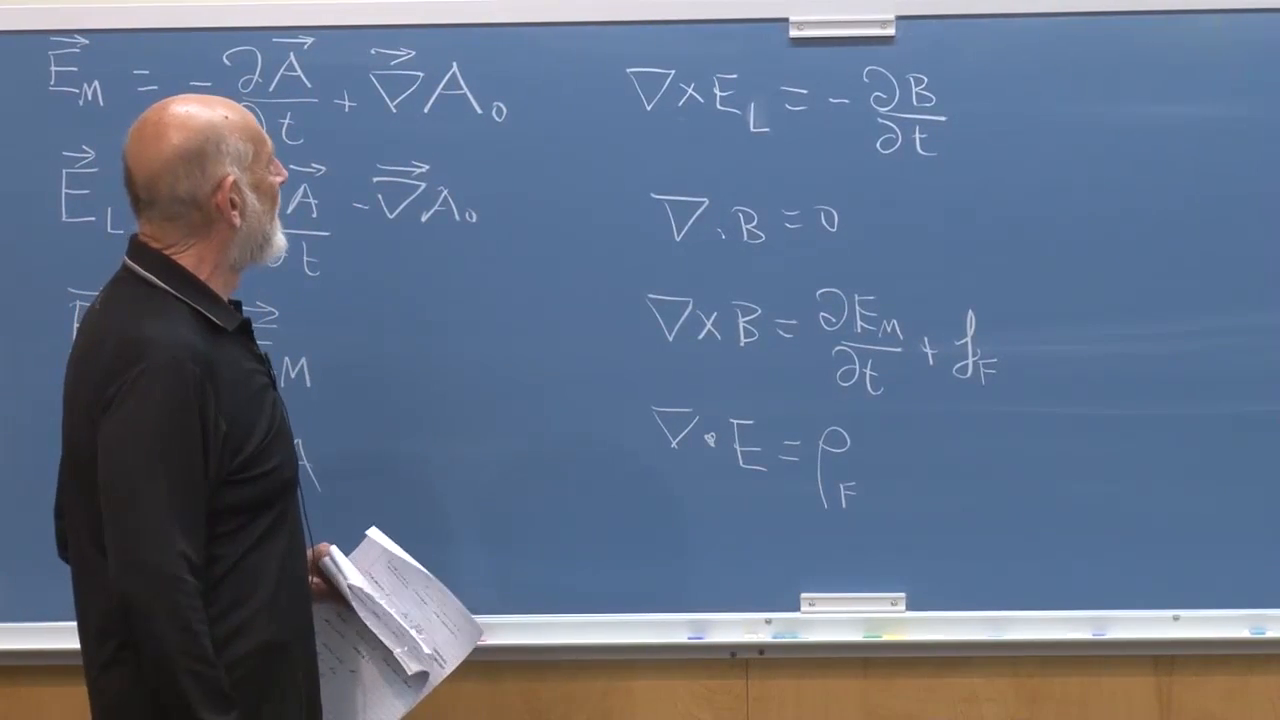
\includegraphics[width=\linewidth]{lecture_10_figure_01.png}
\caption{マクスウェル--フランクリン規約と講義の規約の完全な板書比較。}
\par\smallskip
\textit{講義フレーム：00：07：10。}
\end{figure}

どちらの辞書を選ぶかに、測定可能なものは何も依存しない。重要なのは一貫性であり、とくに計算された場を公表された実験値と比較する場合にそうである。笑い話のような話だが、そのような直接的な数値比較は講師自身の仕事ではごくまれにしか生じなかったため、逆の符号がクラスが注意を向けるまで気づかれずに残っていた。本章の後半の電磁気計算には、標準的な場
\(\mathbf E\equiv\mathbf E_M\)
を用いる。

\section{運動量と呼ばれる三つの異なる量}

\emph{運動量}という語をここで解きほぐさなければならない。力学的運動量、正準運動量、ネーター運動量は簡単な問題では一致することがあるが、それらは一つの量の三つの記述ではない。一般の系では、異なる数値を持ちうる。

\subsection{力学的運動量}

全質量\(M\)の物体について、力学的運動量は
\begin{equation}
\mathbf P_{\mathrm{mech}}=M\dot{\mathbf X}_{\mathrm{cm}}.
\label{eq:mechanical-momentum}
\end{equation}
である。一つの粒子については、\(\mathbf X_{\mathrm{cm}}\)は単にその位置である。複合体については、重心という限定が本質的である。

\begin{figure}[H]
\centering
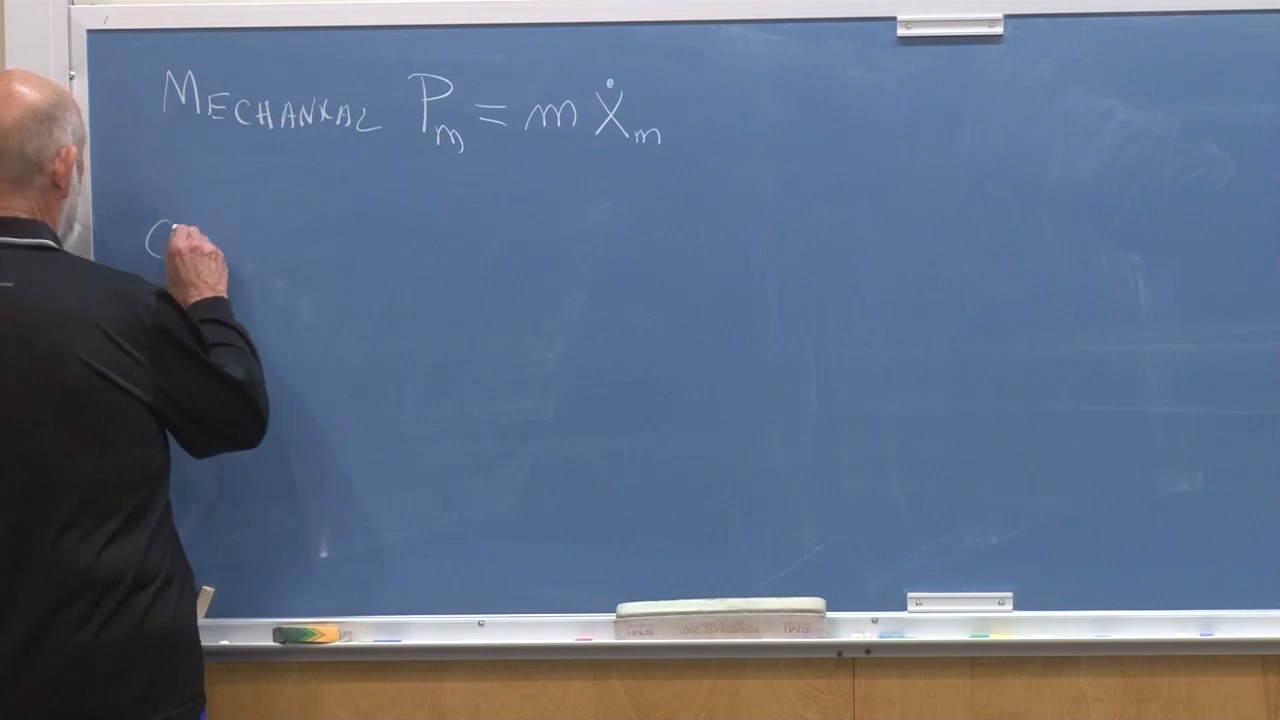
\includegraphics[width=\linewidth]{lecture_10_figure_02.png}
\caption{質量に重心速度を掛けたものとして導入される力学的運動量。}
\par\smallskip
\textit{講義フレーム：00：11：15。}
\end{figure}

\subsection{正準運動量}

力学が
\(L(q_i,\dot q_i)\)
で記述されるとする。\(q_i\)に共役な正準運動量は
\begin{equation}
p_i=\frac{\partial L}{\partial\dot q_i}.
\label{eq:canonical-momentum}
\end{equation}
である。
\begin{equation}
L=\frac12 m\dot{\mathbf x}^{\,2}-V(\mathbf x),
\label{eq:simple-particle-lagrangian}
\end{equation}
に対しては\(\mathbf p=m\dot{\mathbf x}\)が得られるので、正準運動量と力学的運動量はたまたま一致する。

\begin{figure}[H]
\centering
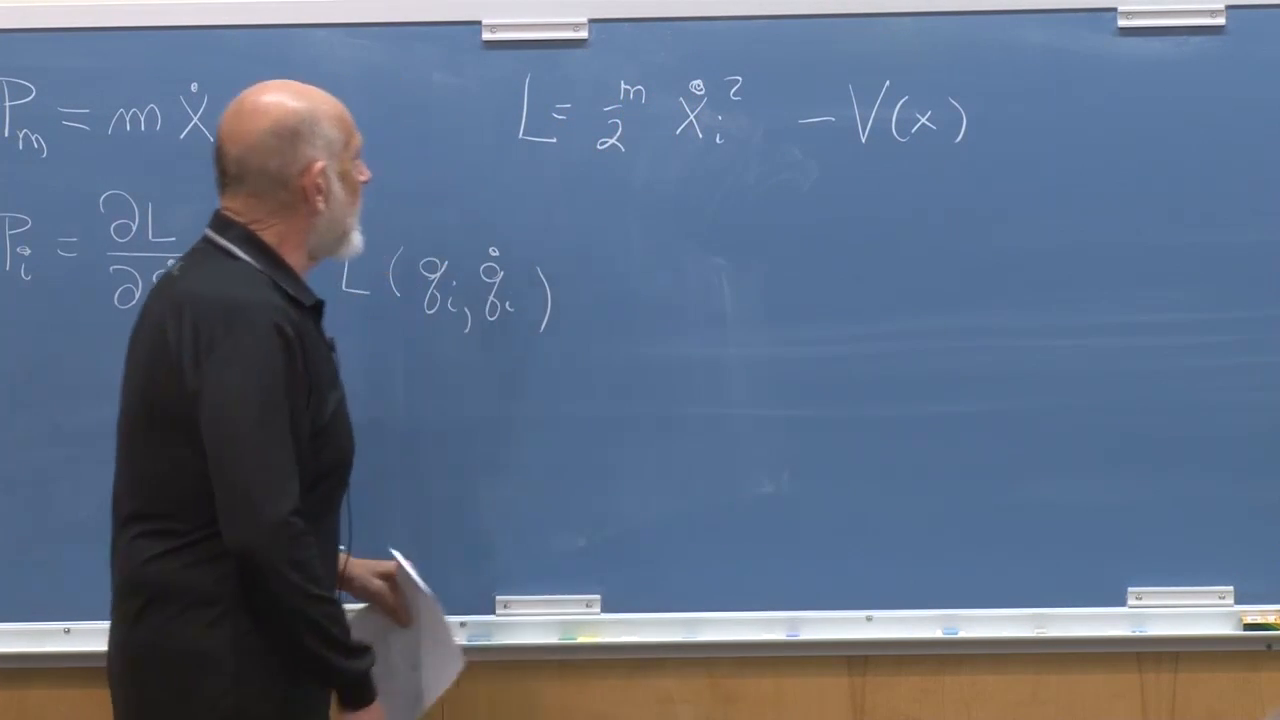
\includegraphics[width=\linewidth]{lecture_10_figure_03.png}
\caption{単純な粒子のラグランジアンの隣に示された力学的運動量と正準運動量。}
\par\smallskip
\textit{講義フレーム：00：13：40。}
\end{figure}

磁場中の荷電粒子が有用な反例である。板書された符号の規約では
\begin{equation}
L=\frac12m\dot{\mathbf x}^{\,2}-V(\mathbf x)
  -e\,\dot{\mathbf x}\cdot\mathbf A(\mathbf x),
\label{eq:magnetic-particle-lagrangian}
\end{equation}
であり、したがって
\begin{equation}
p_i=m\dot x_i-eA_i.
\label{eq:magnetic-canonical-shift}
\end{equation}
となる。電荷または相互作用項の規約を変えれば表示される符号は変わるが、教訓は変わらない。正準運動量はベクトルポテンシャルの寄与を含み、単なる\(m\dot x_i\)ではない。ハミルトンの方程式は正準変数を用いる。後で場に依存する項を方程式の反対側へ移し、ニュートン的な見かけの加速度を取り戻すことはできるが、その並べ替えは定義を変えない。

\begin{figure}[H]
\centering
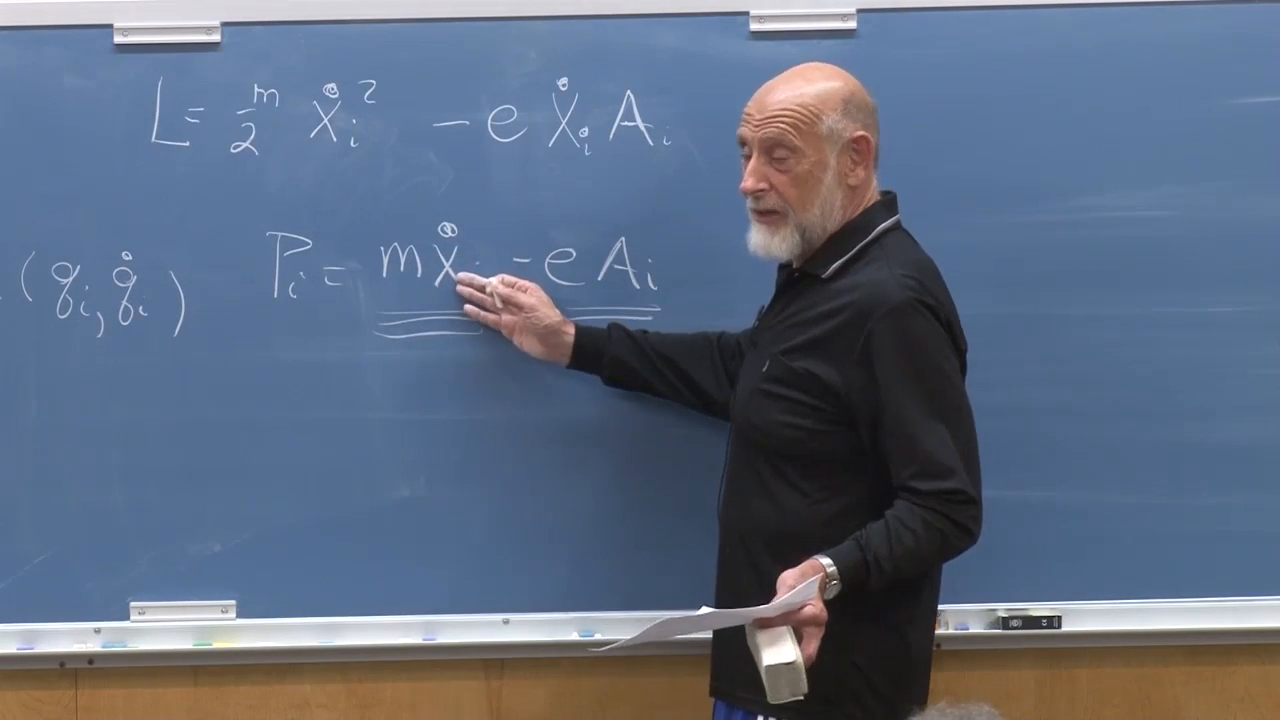
\includegraphics[width=\linewidth]{lecture_10_figure_04.png}
\caption{ベクトルポテンシャルの項が正準運動量を力学的運動量からずらす。}
\par\smallskip
\textit{講義フレーム：00：15：50。}
\end{figure}

\subsection{ネーター運動量}

第三の運動量は、空間並進不変性に対応する保存電荷である。微小な対称性
\begin{equation}
q_i\longrightarrow q_i+\delta q_i
\end{equation}
がラグランジアンを不変に保つとき、ネーターの定理は、微小パラメータの規格化を除いて、
\begin{equation}
Q=\sum_i p_i\,\delta q_i.
\label{eq:noether-charge-mechanics}
\end{equation}
を与える。ここに現れる\(p_i\)は正準運動量である。対称性が一様並進であり、正準運動量がたまたま力学的運動量に等しいならば、\(Q\)はよく知られた全運動量に帰着する。より単純でない系では、その一致は仮定されるのではなく証明されなければならない。

\begin{figure}[H]
\centering
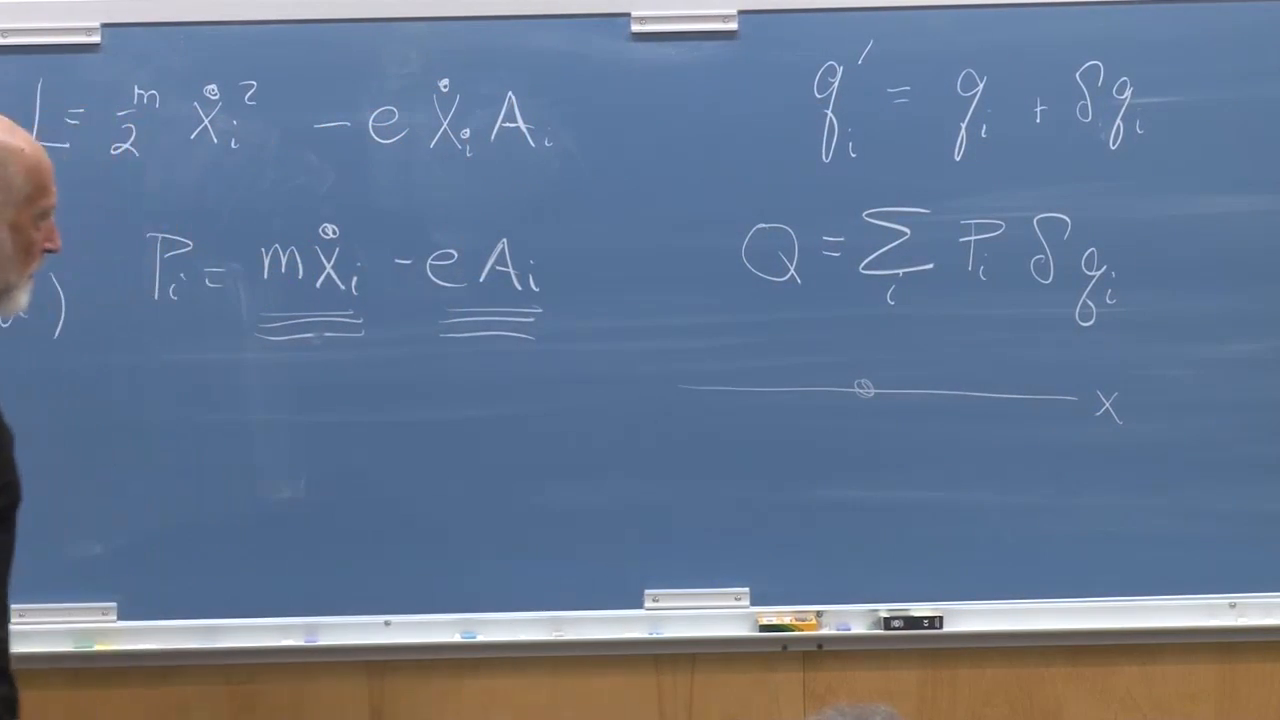
\includegraphics[width=\linewidth]{lecture_10_figure_05.png}
\caption{正準運動量と座標の微小変化から組み立てられたネーター電荷。}
\par\smallskip
\textit{講義フレーム: 00:19:00.}
\end{figure}

\section{ハミルトニアンとしてのエネルギー}

空間並進は運動量を導き、時間並進はエネルギーを導く。ラグランジアンが時間に陽に依存しないならば、ハミルトニアン
\begin{equation}
H=\sum_i p_i\dot q_i-L
\label{eq:hamiltonian-definition}
\end{equation}
は保存される。これはラグランジアンのルジャンドル変換であり、符号を目で見て変える規則ではない。

\begin{figure}[H]
\centering
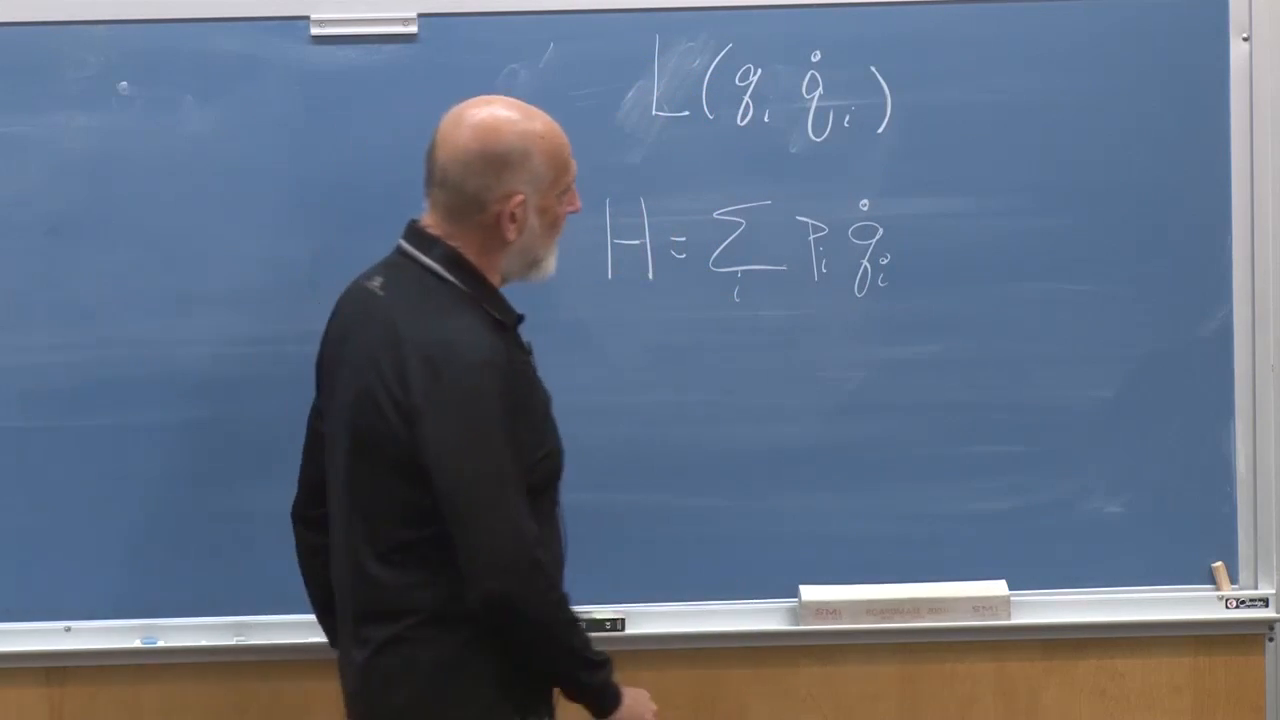
\includegraphics[width=\linewidth]{lecture_10_figure_06.png}
\caption{一般のラグランジアンのルジャンドル変換として書かれたハミルトニアン。}
\par\smallskip
\textit{講義フレーム: 00:22:55.}
\end{figure}

一粒子の例では、
\begin{align}
p&=m\dot x,
\nonumber\\
H&=p\dot x-L\\
&=m\dot x^2
  -\left(\frac12m\dot x^2-V(x)\right)\\
&=\frac12m\dot x^2+V(x).
\label{eq:particle-hamiltonian}
\end{align}
したがって、ラグランジアンは運動エネルギーからポテンシャルエネルギーを引いたものであり、ハミルトニアンは運動エネルギーにポテンシャルエネルギーを加えたものである。

\begin{figure}[H]
\centering
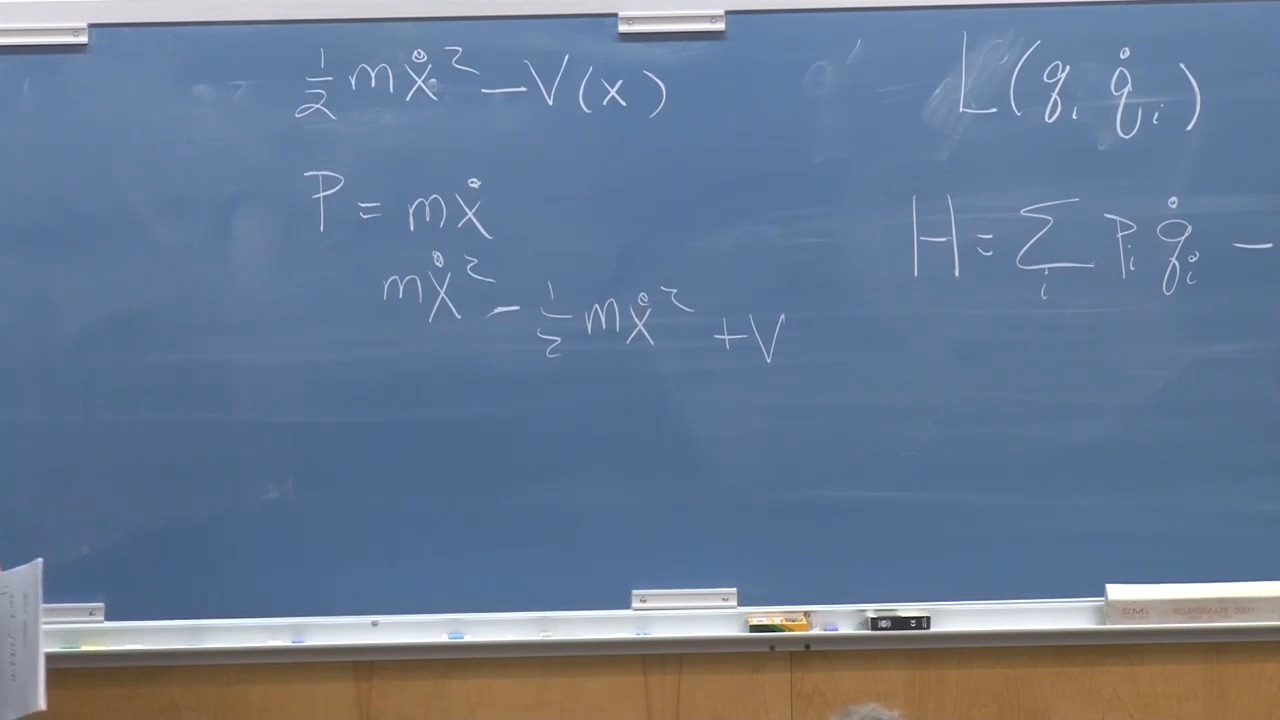
\includegraphics[width=\linewidth]{lecture_10_figure_07.png}
\caption{\(H=T+V\)が\(H=p\dot x-L\)からどのように導かれるかを示す粒子の計算。}
\par\smallskip
\textit{講義フレーム: 00:24:20.}
\end{figure}

すべての速度依存性が慣習的な正の二次の運動項であり、残りが速度を含まないとき、非速度部分の符号を逆にすることでハミルトニアンを読み取ることができる。この近道は繰り返し用いられる。それが安全なのは、手元の例においてルジャンドル変換がこの単純な形をとるからにすぎない。

\section{場は連続的に多数の座標をもつ力学系である}

場の理論の力学的構造を明らかにするために、一つの慣性系を選び、すべての行が明白なローレンツ共変性を示すことを一時的に要求するのをやめる。古典力学には時間軸と座標\(q_i(t)\)がある。スカラー場には時間軸と座標\(\phi(\mathbf x,t)\)がある。離散的なラベル\(i\)は、単に連続的なラベル\(\mathbf x\)になったのである:
\begin{equation}
q_i(t)\quad\longrightarrow\quad\phi(\mathbf x,t).
\label{eq:discrete-to-field}
\end{equation}
各空間点における場の値が一つの自由度である。ここで\(\mathbf x\)はどの自由度を指すかを示すラベルであり、それ自体が一般化座標ではない。

\begin{figure}[H]
\centering
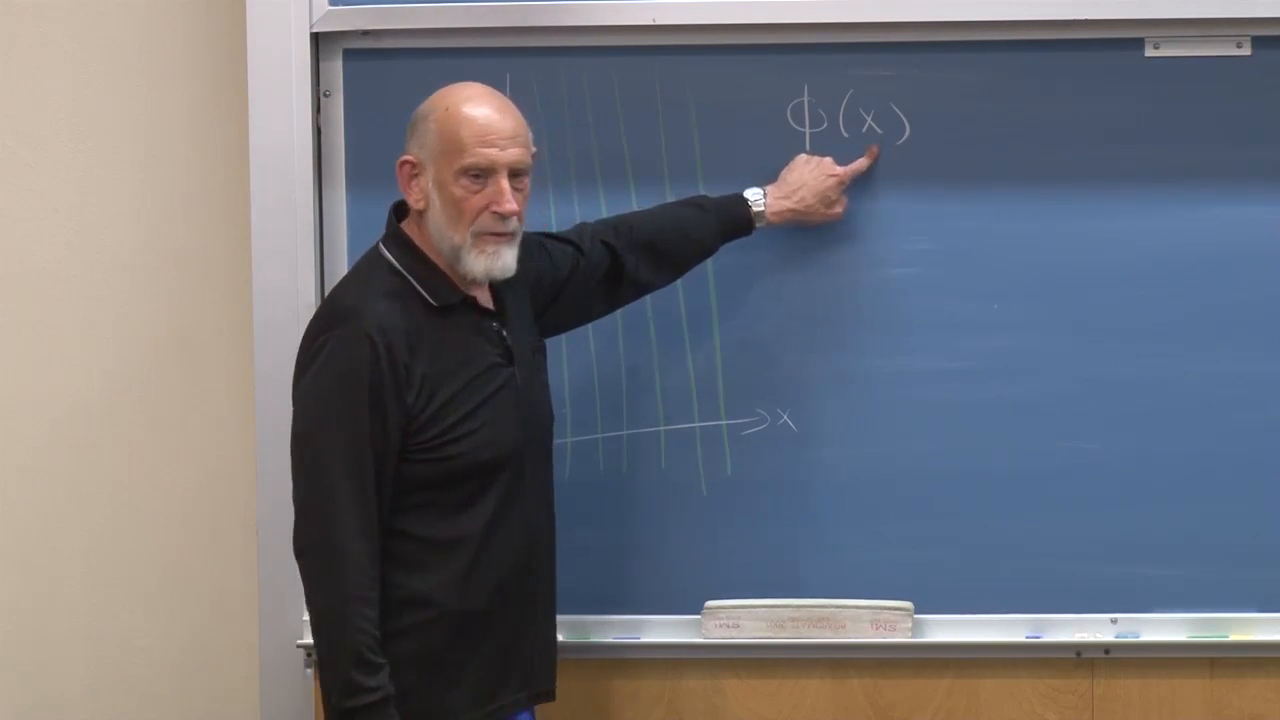
\includegraphics[width=\linewidth]{lecture_10_figure_08.png}
\caption{各点における場の値を別個の力学的自由度として表示するために用いられる空間的格子。}
\par\smallskip
\textit{講義フレーム: 00:30:15.}
\end{figure}

\begin{classroomqa}
\audiencequestion{なぜ最初から場を
\(\phi(\mathbf x,t)\)と書かないのか?}
\lecturerresponse{それが完全な記法である。一時的な
\(\phi(\mathbf x)\)は、すべての\(q_i\)が時間に依存することを念頭に置きながらしばしば\(q_i\)と書くのと同様に、共通の時間引数を省略している。ラベル\(i\)、あるいは今では\(\mathbf x\)が、どの自由度が議論されているかを教えてくれる。\lecturetimestamp{00:32:43}}
\end{classroomqa}

\begin{classroomqa}
\audiencequestion{隣接点における場の値は本当に独立な座標なのか? 何が連続性を課すのか?}
\lecturerresponse{それらは独立な正準座標である。滑らかさは隣接する値を同一視することによって課されるのではなく、力学的に選択される。ハミルトニアンは正の勾配エネルギー項を含むので、ますます小さな距離にわたる固定された跳びはますます多くのエネルギーを要する。したがって、有限エネルギーの配置は連続極限において滑らかになる。\lecturetimestamp{00:33:09}}
\end{classroomqa}

空間微分は隣接する自由度の間の結合を明示する。間隔\(\epsilon\)の格子上では、
\begin{equation}
\partial_x\phi(x,t)
  =\lim_{\epsilon\to0}
   \frac{\phi(x+\epsilon,t)-\phi(x,t)}{\epsilon}.
\label{eq:field-finite-difference}
\end{equation}
これは近接する二つの座標に依存するが、一般化速度を含まない。力学的類推では、これはラグランジアンの座標依存性に属し、\(\dot q_i\)依存性には属さない。

\begin{figure}[H]
\centering
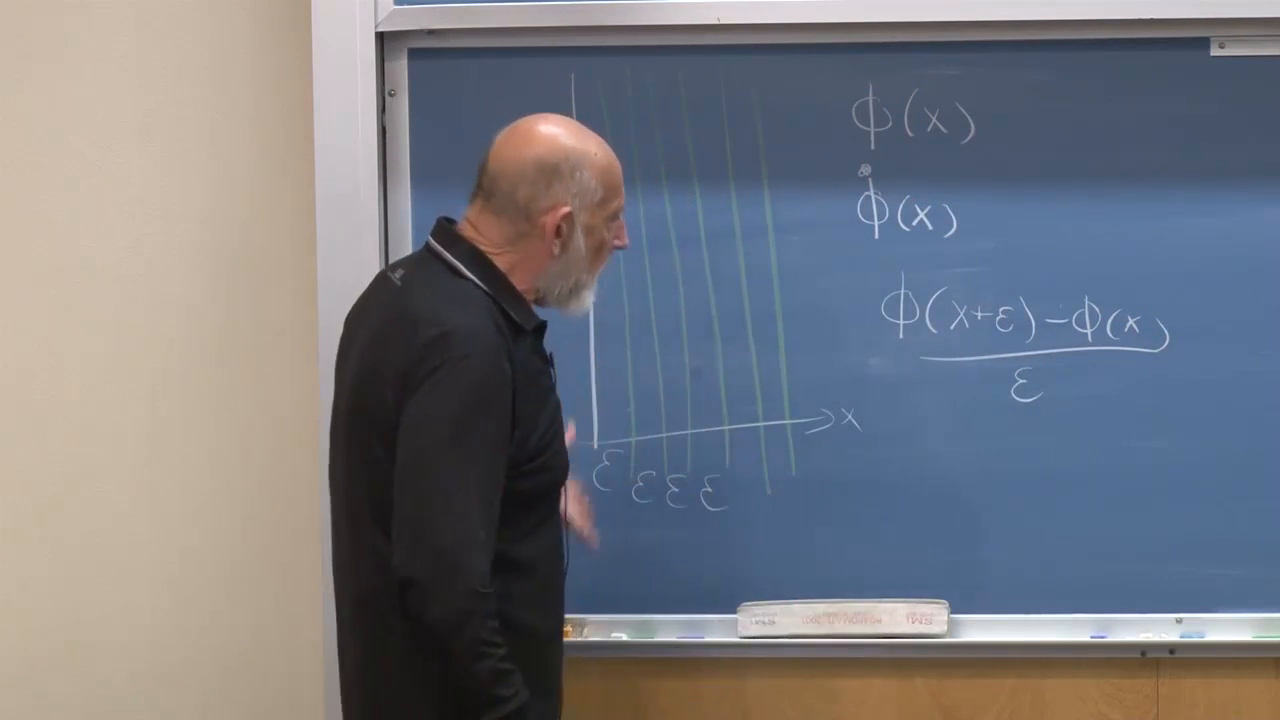
\includegraphics[width=\linewidth]{lecture_10_figure_09.png}
\caption{格子上の隣接場の差として再構成された空間微分。}
\par\smallskip
\textit{講義フレーム: 00:31:40.}
\end{figure}

作用は今や陽に力学的な形で書くことができる:
\begin{align}
S&=\int dt\,L,
\nonumber\\
L&=\int d^3x\,
\mathcal L\!\left(
\phi,\dot\phi,\boldsymbol{\nabla}\phi
\right),
\nonumber\\
S&=\int dt\,d^3x\,
\mathcal L\!\left(
\phi,\dot\phi,\boldsymbol{\nabla}\phi
\right).
\label{eq:field-action-split}
\end{align}
筆記体の\(\mathcal L\)はラグランジアン密度である。これを空間にわたって積分すると、時間にわたって積分される通常のラグランジアンが得られる。局所的な理論は、各点をその点における場とその導関数を通じてのみ結合する。時間と空間を分けることはローレンツ共変性を一時的に隠すが、力学を透明にする。

\begin{figure}[H]
\centering
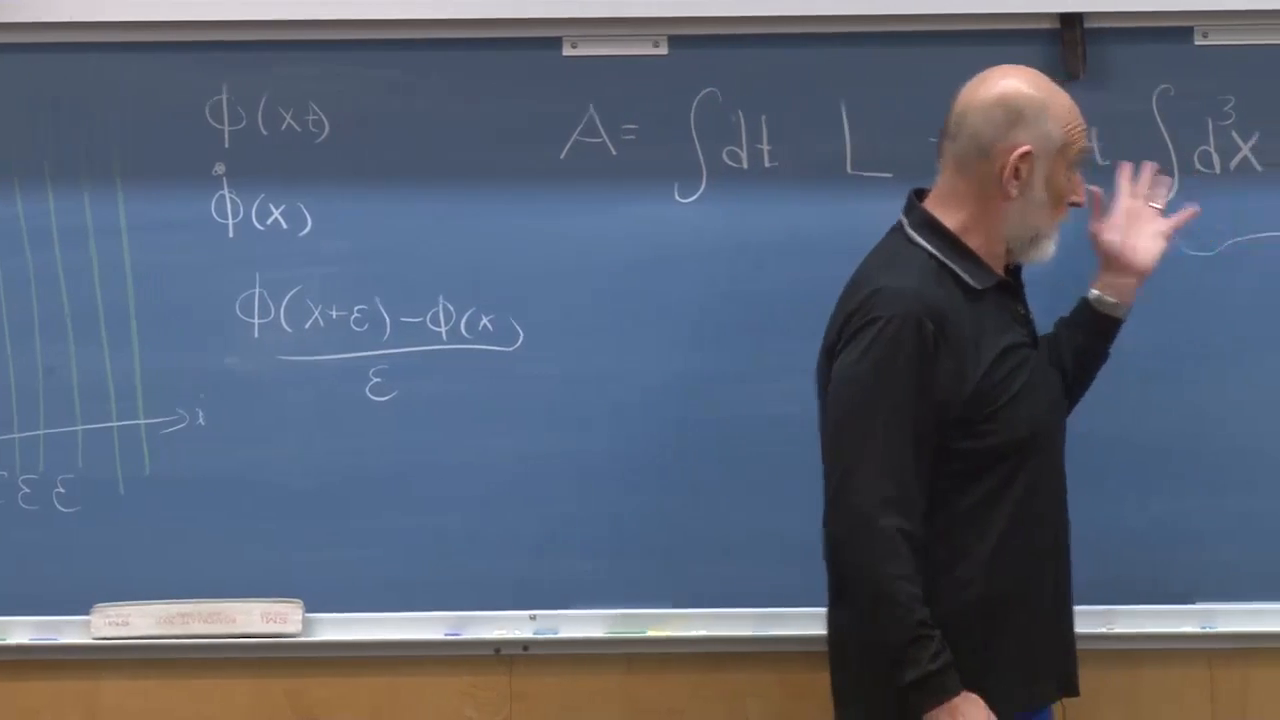
\includegraphics[width=\linewidth]{lecture_10_figure_10.png}
\caption{場の作用を時間積分とラグランジアン密度の空間積分に分けたもの。}
\par\smallskip
\textit{講義フレーム：00：36：40。}
\end{figure}

\section{正準場の運動量とハミルトニアン密度}

場の座標の速度とは\(\dot\phi(\mathbf x,t)\)、すなわち一つの固定点において場が時間的に変化する割合である。それは一つの空間点から別の空間点への運動ではない。したがって場に共役な正準運動量もまたそれ自体が場であり、
\begin{equation}
\Pi(\mathbf x,t)
 =\frac{\partial\mathcal L}{\partial\dot\phi(\mathbf x,t)}.
\label{eq:field-canonical-momentum}
\end{equation}
複数の場\(\phi_a\)に対しては、それぞれに一つの運動量場\(\Pi_a\)が存在する。

ルジャンドル変換における離散和は空間積分になる：
\begin{align}
H
 &=\int d^3x\,
   \left[\Pi\dot\phi-\mathcal L\right]
  =\int d^3x\,\mathcal H,
\nonumber\\
\mathcal H
 &=\Pi\dot\phi-\mathcal L .
\label{eq:field-hamiltonian-density}
\end{align}
積分の内側の量がエネルギー密度である。

\begin{figure}[H]
\centering
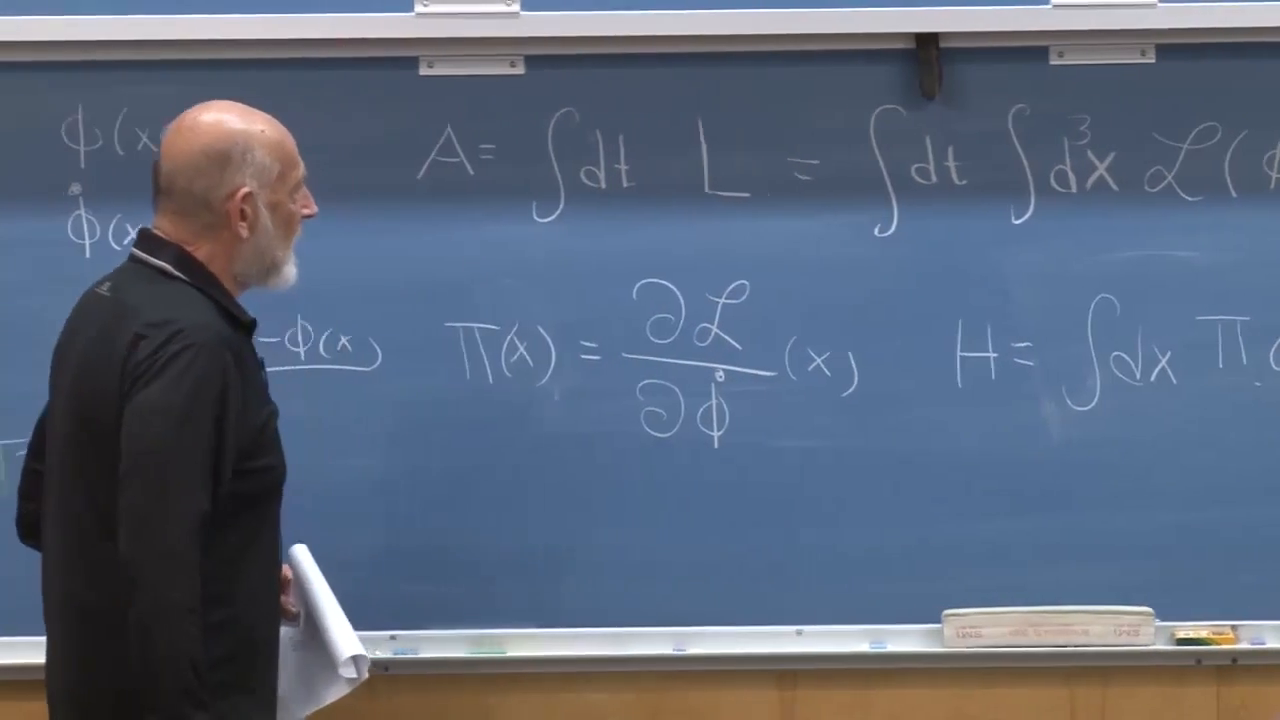
\includegraphics[width=\linewidth]{lecture_10_figure_11.png}
\caption{場のルジャンドル変換と、その局所エネルギー密度の積分としての解釈。}
\par\smallskip
\textit{講義フレーム：00：42：40。}
\end{figure}

\begin{classroomqa}
\audiencequestion{なぜ一点における\(\dot\phi\)に関する全ラグランジアンの微分を、その点における局所密度の微分で置き換えてよいのか。}
\lecturerresponse{空間積分を連続的な和とみなせばよい。ここで用いている局所性の仮定の下では、速度\(\dot\phi(\mathbf x)\)は同じ点に属する項にのみ現れる。その特定の速度に関する微分は他のすべての項を消し去る。空間微分は隣接する場の値を結合しうるが、この理論では隣接する時間微分を持ち込まない。\lecturetimestamp{00:51:56}}
\end{classroomqa}

\subsection{スカラー場}

一次元空間において、
\begin{equation}
\mathcal L
 =\frac12\dot\phi^2
  -\frac12(\partial_x\phi)^2
  -V(\phi).
\label{eq:scalar-field-lagrangian}
\end{equation}
を取る。これは先に用いたローレンツスカラーの非共変的な表示である。時間微分と空間微分の間の相対的な負符号はミンコフスキー計量に由来する。正準運動量は
\begin{equation}
\Pi=\dot\phi,
\label{eq:scalar-pi}
\end{equation}
であり、ハミルトニアンは
\begin{equation}
H=\int dx\,
\left[
\frac12\dot\phi^2
+\frac12(\partial_x\phi)^2
+V(\phi)
\right].
\label{eq:scalar-field-hamiltonian}
\end{equation}
となる。計算の途中でポテンシャルは一時的に\(V(x)\)と呼ばれたが、クラスはそれを\(V(\phi)\)に訂正した。それは場を通じて間接的に位置に依存しうるが、並進不変な理論においては規定された外部の\(x\)依存性を持たない。

\begin{figure}[H]
\centering
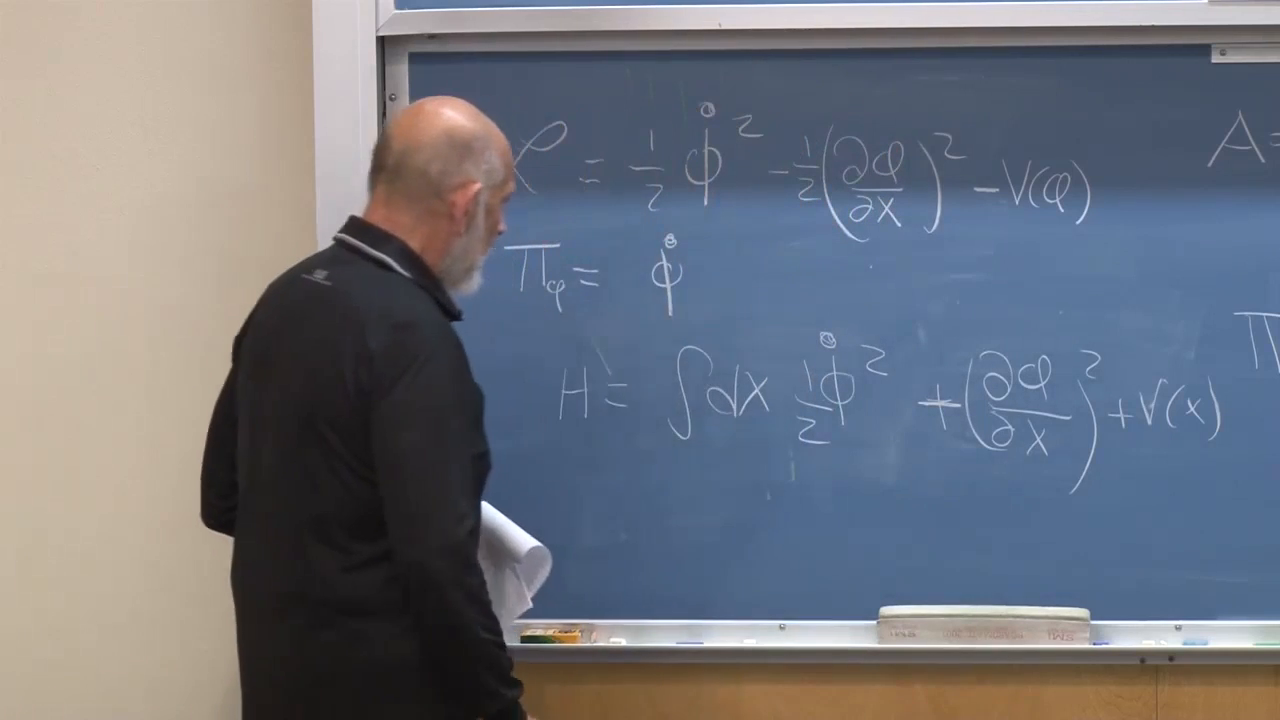
\includegraphics[width=\linewidth]{lecture_10_figure_12.png}
\caption{スカラーのラグランジアン密度、共役運動量、正のハミルトニアンを一つの板書にまとめたもの。}
\par\smallskip
\textit{講義フレーム：00：47：05。}
\end{figure}

時間微分を含まない部分全体がポテンシャルエネルギーの役割を果たす。それには\(V(\phi)\)と勾配エネルギー\(\frac12(\partial_x\phi)^2\)の両方が含まれる。ラグランジアンはどちらの符号も取りうるが、安定なエネルギーは下に有界であるべきである。

\begin{classroomqa}
\audiencequestion{ポテンシャル\(V(\phi)\)は負であってよいか。}
\lecturerresponse{よい。有限な下界を持つならば、古典場の方程式を変えずにその最小値がゼロになるよう定数を加えることができる。下に有界でないポテンシャルは不安定性を表す。場はそのエネルギーを限りなく下げることができる。安定な真空は、ずらしたポテンシャルの最小値に位置する定数場である。
\lecturetimestamp{00:49:03}}
\end{classroomqa}

先の連続性に関する問いは今や定量的に答えられる。格子間隔\(\epsilon\)にわたる跳び\(\Delta\phi\)は
\begin{equation}
\frac12(\partial_x\phi)^2
\sim\frac12\left(\frac{\Delta\phi}{\epsilon}\right)^2.
\label{eq:gradient-cost}
\end{equation}
に寄与する。\(\epsilon\to0\)のとき、固定された跳びはいくらでも大きなエネルギー密度を与える。したがって有限のエネルギーはぎざぎざした配置を抑圧する。

\begin{figure}[H]
\centering
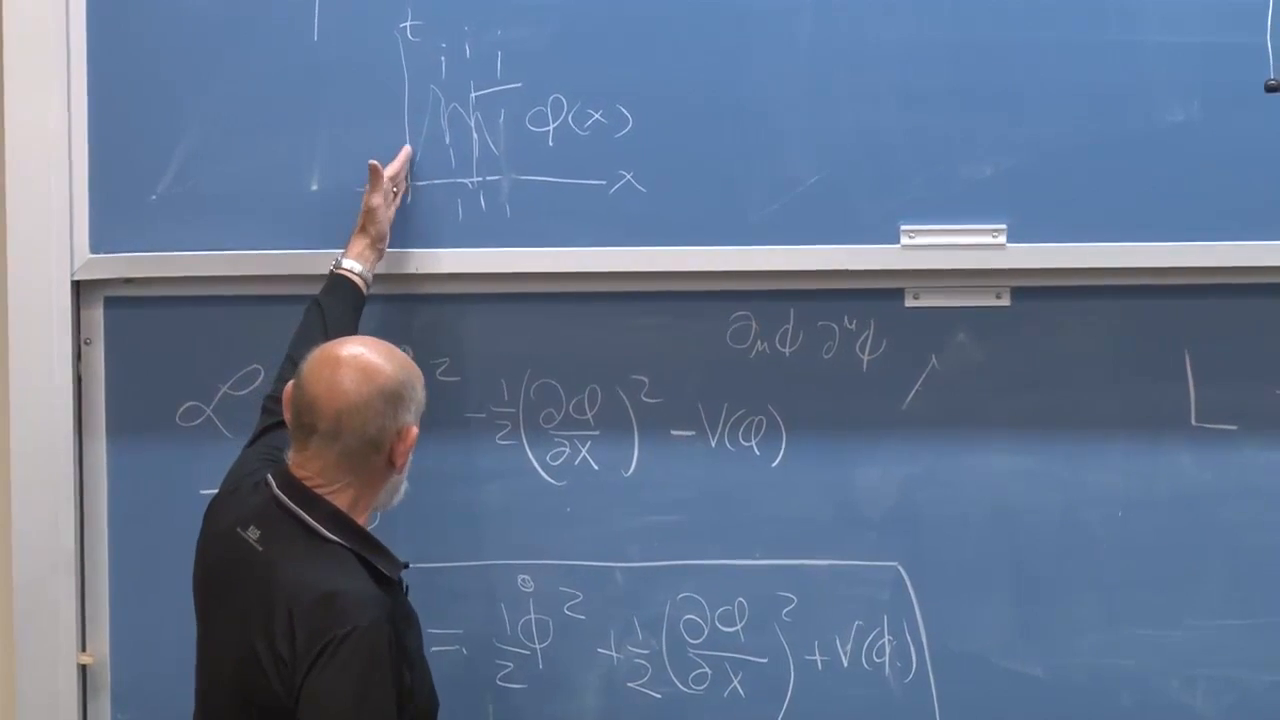
\includegraphics[width=\linewidth]{lecture_10_figure_13.png}
\caption{スカラーのエネルギー公式を保持しつつ、板書のスケッチで滑らかな場と急激な変化を対比したもの。}
\par\smallskip
\textit{講義フレーム：00：54：20。}
\end{figure}

\section{局所エネルギーと\texorpdfstring{\(T^{00}\)}{T00}}

エネルギー密度は簡潔な名を与えられる：
\begin{equation}
T^{00}=\mathcal H=\Pi\dot\phi-\mathcal L.
\label{eq:T00-definition}
\end{equation}
二つのゼロ添字は二つの別個の主張を表す。エネルギーはエネルギー--運動量四元ベクトルの時間成分\(P^0\)であり、一方密度は保存流の時間成分である。したがって\(T^{00}\)は四元運動量の時間成分の密度である。

\begin{figure}[H]
\centering
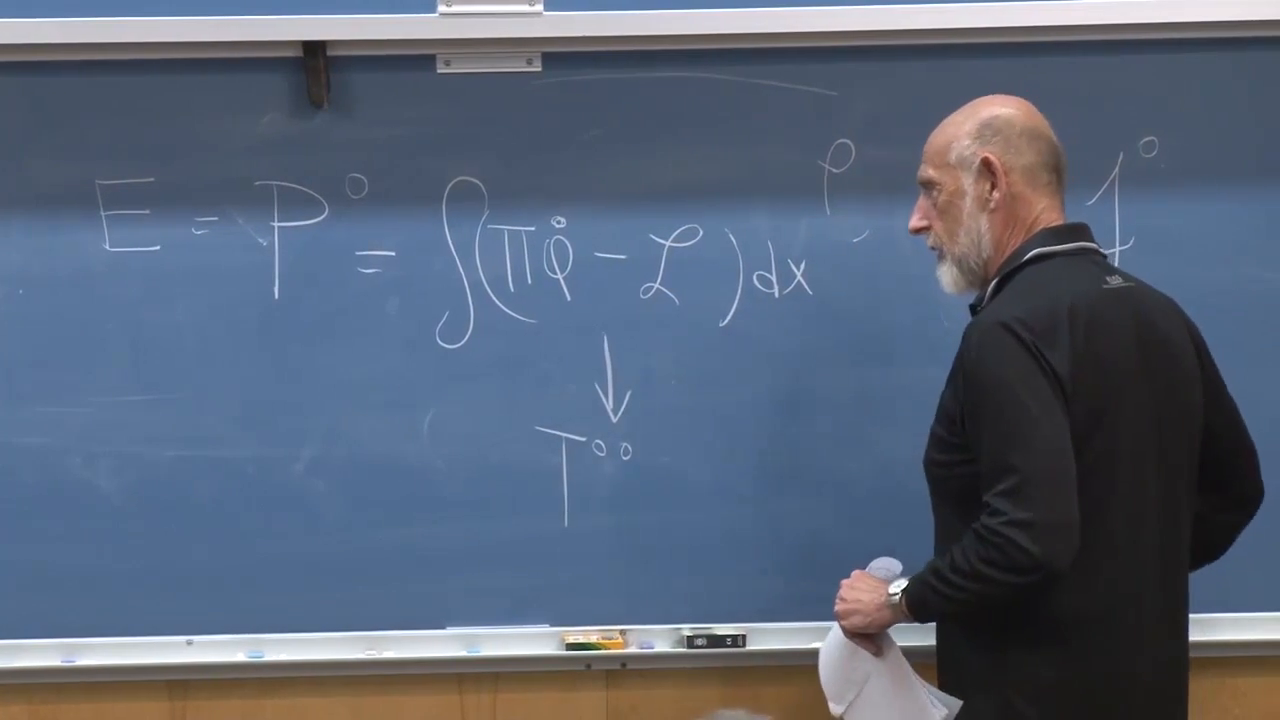
\includegraphics[width=\linewidth]{lecture_10_figure_14.png}
\caption{場のエネルギーを局所的に書き、\(T^{00}\)と同定したもの。}
\par\smallskip
\textit{講義フレーム：01：00：00。}
\end{figure}

相対論的な局所理論における保存は、単に一つの大域的な数が変わらないという主張ではない。エネルギーが実験室で消えてアルファ・ケンタウリに現れることはできない。領域内部の変化はその境界を通る流束によって説明されねばならない。局所的な形では、
\begin{equation}
\partial_\mu T^{\mu\nu}=0,
\label{eq:stress-energy-continuity}
\end{equation}
であるから、第一の添字は密度または流束の方向を表し、第二の添字はどの成分\(P^\nu\)が輸送されているかを表す。

\begin{classroomqa}
\audiencequestion{\(T^{00}\)を密度と呼ぶということは、全エネルギーがそれを積分して得られるという意味か。}
\lecturerresponse{そのとおりである：
\(E=P^0=\int d^3x\,T^{00}\)。局所密度は場のルジャンドル変換における被積分関数である。ある場所でのその変分は、隣接する場所を通るエネルギー流によって釣り合っている。\lecturetimestamp{00:59:06}}
\end{classroomqa}

\section{空間並進からの運動量密度}

再びネーターの公式に戻り、今度は離散的な和を空間積分で置き換える。\(m\)方向への微小並進の下で、場は次で変化する：
\begin{equation}
\delta\phi
  =\phi(\mathbf x)-\phi(\mathbf x-\boldsymbol{\epsilon})
  =\epsilon^m\partial_m\phi+O(\epsilon^2),
\label{eq:translated-field-change}
\end{equation}
ここでは黒板で用いた受動的規約をとっている。能動的並進と受動的並進を入れ替えると全体の符号が反転するが、物理的な生成子はその規約をひとたび選べば確定する。\(\epsilon^m\)をくくり出すと、ネーター運動量は次の構造をもつ：
\begin{equation}
P_m\ \propto\ \int d^3x\,\Pi\,\partial_m\phi.
\label{eq:scalar-noether-momentum}
\end{equation}

\begin{figure}[H]
\centering
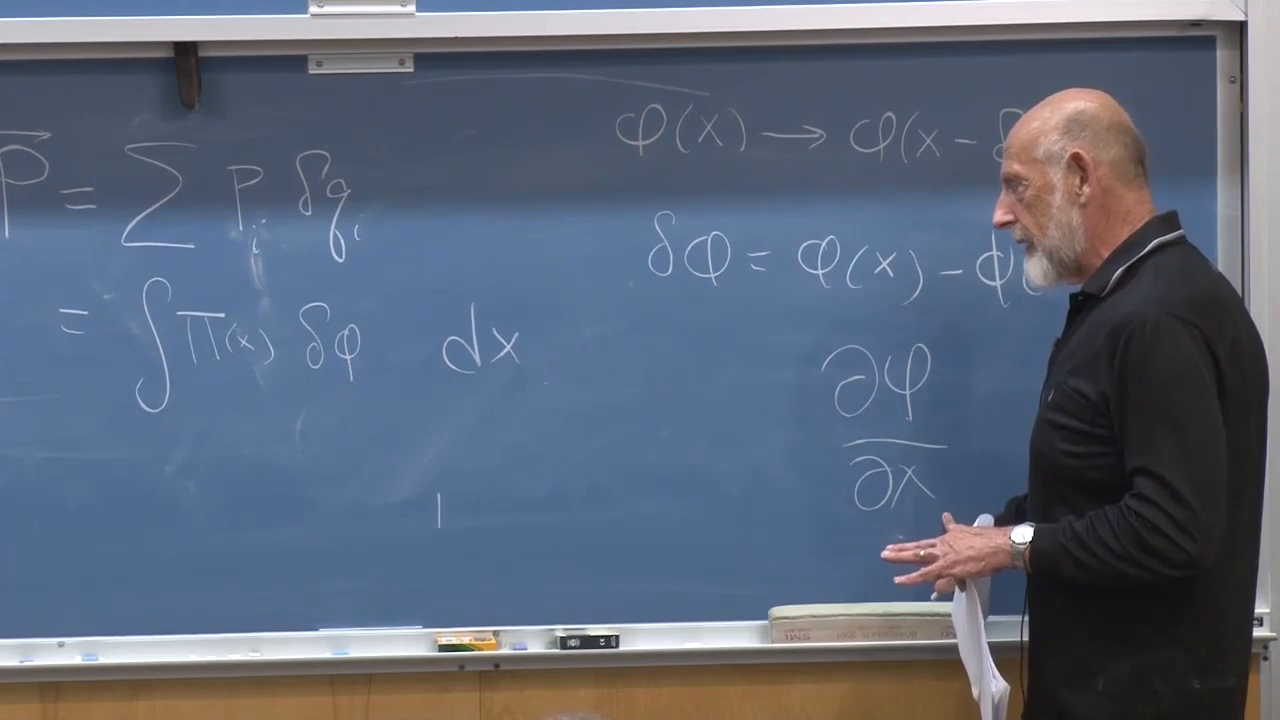
\includegraphics[width=\linewidth]{lecture_10_figure_15.png}
\caption{並進した場のプロファイルと、その無限小変化を測る導関数。}
\par\smallskip
\textit{講義フレーム：01：04：20。}
\end{figure}

\begin{classroomqa}
\audiencequestion{なぜ無限小並進\(\epsilon\)は運動量の公式に残されなかったのか。}
\lecturerresponse{ネーター電荷はまず\(\epsilon\)に比例する形で得られる。運動量はその任意の並進パラメータの係数として定義されるので、\(\epsilon\)は割り出される。保存量に固定した定数を掛けても保存には影響しないが、係数を取り出すことで標準的な規格化が得られる。
\lecturetimestamp{01:04:45}}
\end{classroomqa}

\begin{classroomqa}
\audiencequestion{並進の区間は連続積分における\(dx\)になるのか。}
\lecturerresponse{それらは異なる極限から生じる。測度\(dx\)は、空間的にラベル付けられた自由度の和を積分で置き換えることから来る。並進パラメータ\(\epsilon\)は対称操作を記述するものであり、そのネーター電荷からくくり出される。どちらも中間的な推論においては無限小であるが、果たす役割は異なる。
\lecturetimestamp{01:05:16}}
\end{classroomqa}

講義の記法では、運動量の\(m\)成分の密度は
\begin{equation}
T^{0m}=\Pi\,\partial_m\phi,
\label{eq:scalar-momentum-density}
\end{equation}
であり、並進の符号の規約は了解済みである。スカラー理論では\(\Pi=\dot\phi\)なので、それは\(\dot\phi\,\partial_m\phi\)に比例する。

\begin{figure}[H]
\centering
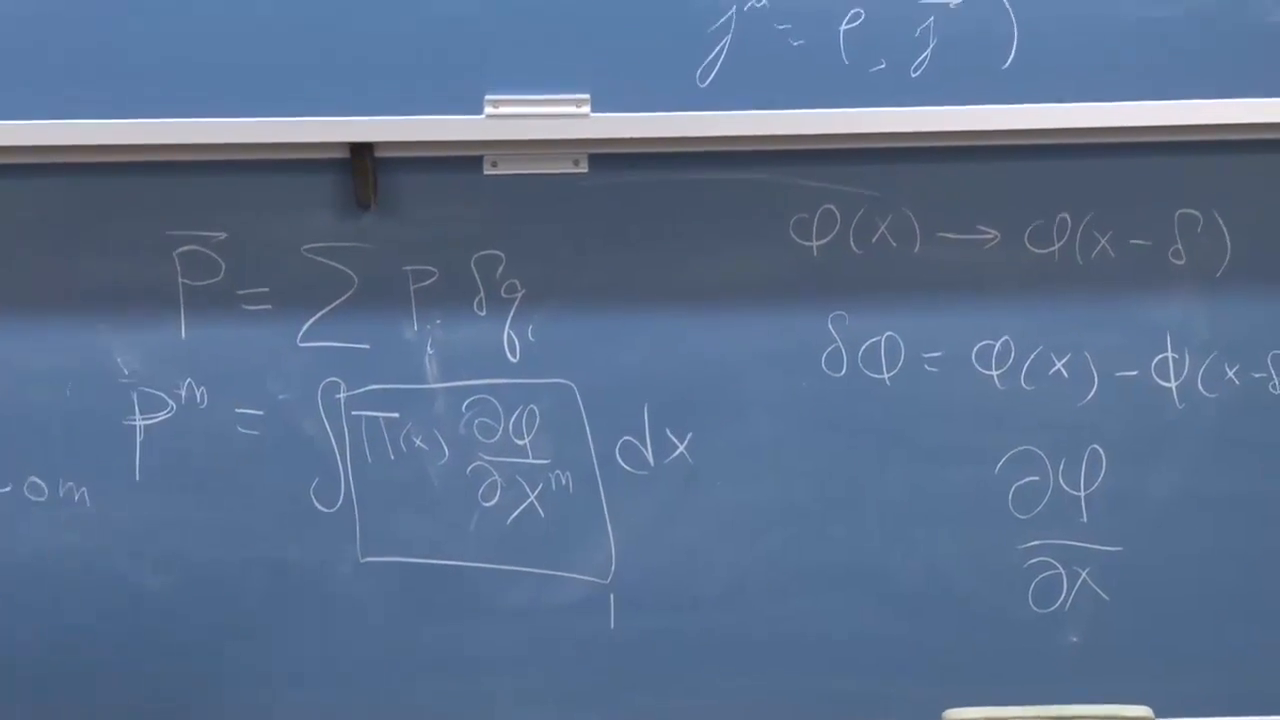
\includegraphics[width=\linewidth]{lecture_10_figure_16.png}
\caption{黒板上のネーター運動量密度\(T^{0m}=\Pi\,\partial_m\phi\)。}
\par\smallskip
\textit{講義フレーム：01：07：10。}
\end{figure}

これは波によって運ばれる文字通りの運動量である。並進不変性は、すべてが並進されるときにのみ適用される：場、粒子、源、そして装置である。自由に吊るされた板に吸収された光パルスは、板に反跳を与える。通常の光ではこの効果はごく小さいが、十分に強力なレーザーは小さな標的を圧縮するのに十分な運動量を伝達しうる。保存される全量は粒子と場の双方に属する。

\subsection{ニュートンの方程式に代わるものは何か。}

~\eqref{eq:scalar-field-lagrangian}式から導かれる場のオイラー--ラグランジュ方程式は
\begin{equation}
\ddot\phi-\nabla^2\phi=-\frac{dV}{d\phi}.
\label{eq:scalar-equation-of-motion}
\end{equation}
である。これはニュートンの法則の場の理論における類似物である。

\begin{figure}[H]
\centering
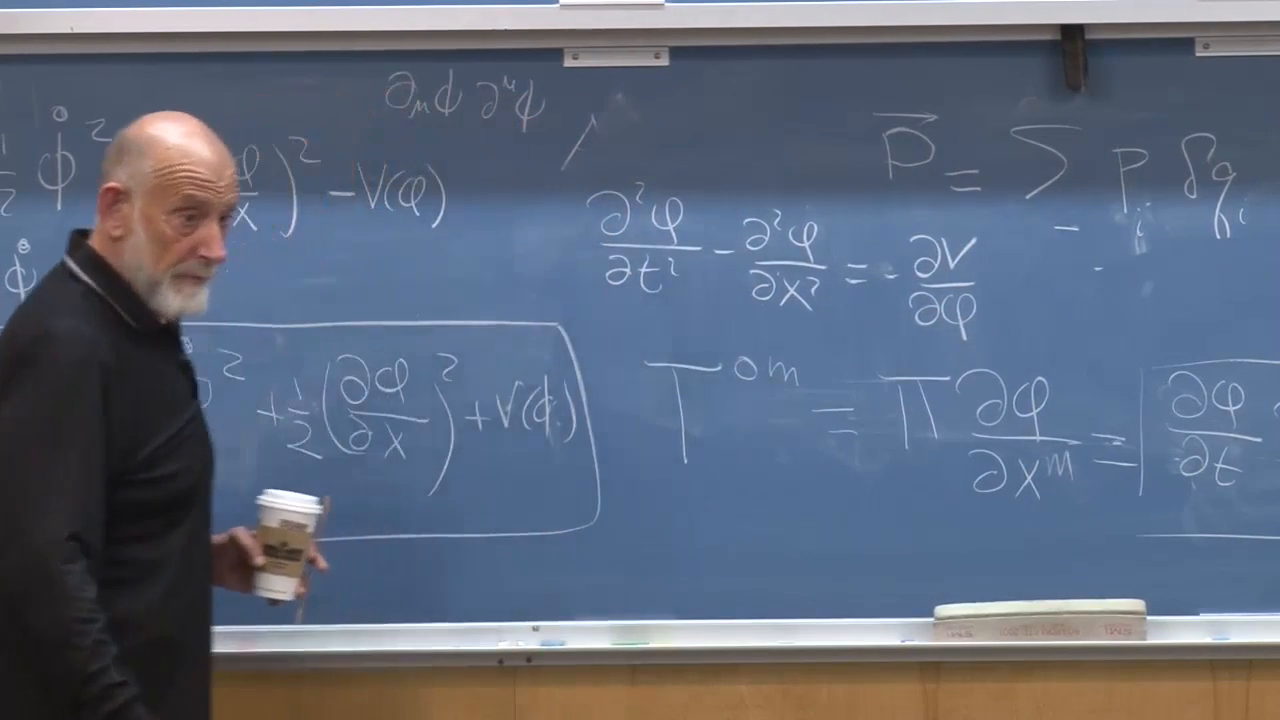
\includegraphics[width=\linewidth]{lecture_10_figure_17.png}
\caption{そのハミルトニアンと運動量密度の隣に表示されたスカラー場の方程式。}
\par\smallskip
\textit{講義フレーム：01：12：55。}
\end{figure}

\begin{classroomqa}
\audiencequestion{場に対するニュートンの法則に対応するものは何か。}
\lecturerresponse{オイラー--ラグランジュ場の方程式がそれである。ここでは力の項\(-V'(\phi)\)をもつ波動方程式である。\(m\ddot x=-V'(x)\)の役割は\(\ddot\phi-\nabla^2\phi=-V'(\phi)\)が担っている。
\lecturetimestamp{01:11:48}}
\end{classroomqa}

\begin{classroomqa}
\audiencequestion{提案された場のラグランジアンが正しいことをどうやって知るのか。すでに場の方程式を知っていなければならないのか。}
\lecturerresponse{どちらの方向も可能である。歴史的には、ニュートンやマクスウェルの場合のように、実験から方程式を推論し、その後で作用を探し求めることがある。現代の理論では、場の内容、局所性、対称性、および少数の許容される項から出発し、方程式を導き、その予言を検証することがしばしばである。表示されたスカラーは基本的な場を記述しうるが、その連続作用が構成粒子から導かれる縄の横変位を記述することも同様に可能である。\lecturetimestamp{01:12:55}}
\end{classroomqa}

\section{時間ゲージにおける電磁場}

すでに求めた成分\(T^{00}\)と\(T^{0m}\)は、エネルギー--運動量テンソルに属する。その残りの成分はエネルギーと運動量の流束を記述する。このテンソルは後に重力の源となるが、電磁気学が直接の例を与える。

基本的な電磁気の座標は4元ポテンシャル\(A_\mu\)である。ゲージ自由度により、\(F_{\mu\nu}\)を変えずに
\begin{equation}
A_\mu\longrightarrow A'_\mu=A_\mu+\partial_\mu S
\label{eq:gauge-transformation-lecture10}
\end{equation}
とできる。\(S\)を
\begin{equation}
\partial_tS=-A_0.
\label{eq:temporal-gauge-choice}
\end{equation}
を満たすように選ぶ。例えば、各固定された空間点で\(A_0\)を時間について積分すればよい。変換後の時間成分は消える：
\begin{equation}
A'_0=A_0+\partial_tS=0.
\label{eq:temporal-gauge}
\end{equation}
これが時間ゲージである。これは\(A_0\)を力学座標のリストから除くが、ガウスの法則は拘束条件として残り、時間に依存しない残余ゲージ自由度も残る。

\begin{figure}[H]
\centering
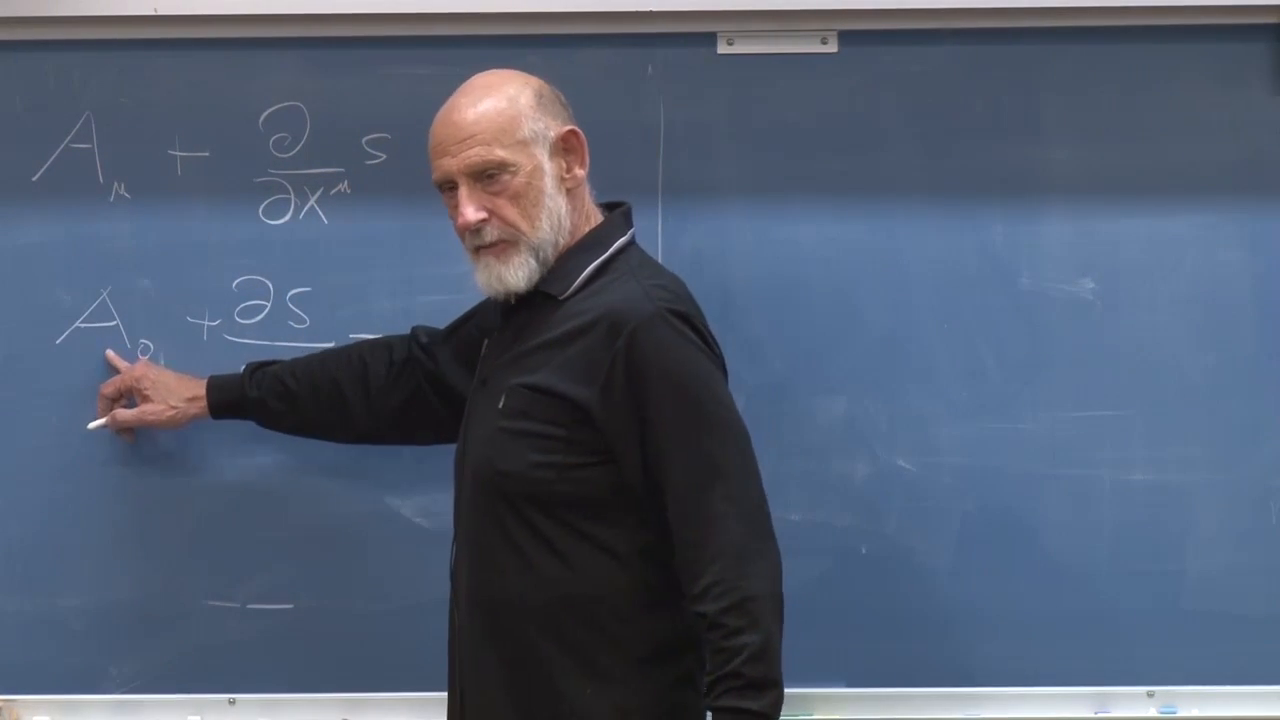
\includegraphics[width=\linewidth]{lecture_10_figure_18.png}
\caption{ゲージ自由度を用いて、\(\partial_tS=-A_0\)を解くことにより\(A_0=0\)を選ぶ。}
\par\smallskip
\textit{講義フレーム：01：20：15。}
\end{figure}

これ以降、\(\mathbf E\)は標準的なマクスウェル場を表すものとする。ゲージ固定の前には、
\begin{equation}
E_m=-\partial_tA_m+\partial_mA_0,
\qquad
\mathbf B=\boldsymbol{\nabla}\times\mathbf A.
\label{eq:E-B-general-potential}
\end{equation}
時間ゲージではこれらは
\begin{equation}
\mathbf E=-\dot{\mathbf A},
\qquad
\mathbf B=\boldsymbol{\nabla}\times\mathbf A.
\label{eq:E-B-temporal-gauge}
\end{equation}
に帰着する。\(\mathbf A\)の時間微分は電場を生じ、空間微分は磁場を生じる。

\begin{figure}[H]
\centering
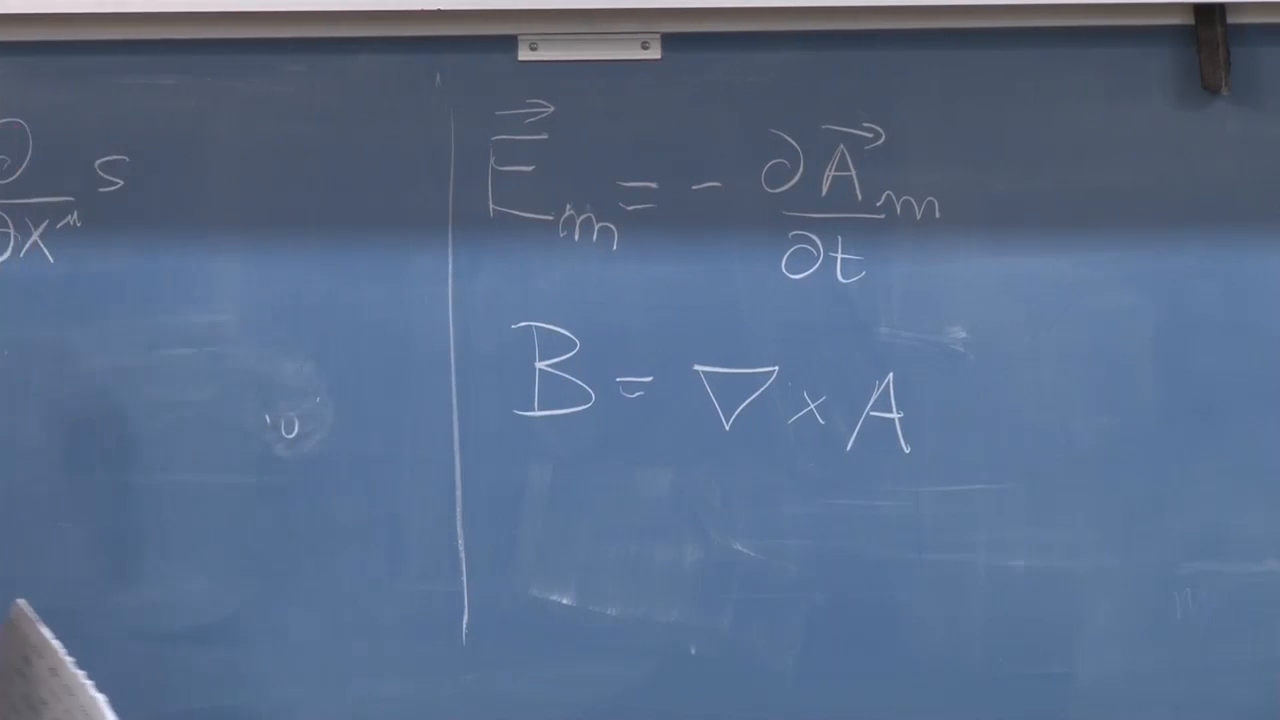
\includegraphics[width=\linewidth]{lecture_10_figure_19.png}
\caption{時間ゲージにおける電場と磁場：
\(\mathbf E=-\dot{\mathbf A}\)および
\(\mathbf B=\nabla\times\mathbf A\)。}
\par\smallskip
\textit{講義フレーム：01：23：50。}
\end{figure}

\section{電磁気の正準運動量とエネルギー}

自由マクスウェルラグランジアン密度は
\begin{equation}
\mathcal L_{\mathrm{EM}}
 =-\frac14F_{\mu\nu}F^{\mu\nu}
 =\frac12\left(\mathbf E^2-\mathbf B^2\right).
\label{eq:maxwell-lagrangian-energy-lecture}
\end{equation}
時間ゲージでは、
\begin{equation}
\mathcal L_{\mathrm{EM}}
 =\frac12\dot{\mathbf A}^{\,2}
  -\frac12(\boldsymbol{\nabla}\times\mathbf A)^2.
\label{eq:maxwell-lagrangian-temporal}
\end{equation}
これはまさにスカラー場のパターンである：時間微分の二乗から空間微分の二乗を引いたものである。

\begin{figure}[H]
\centering
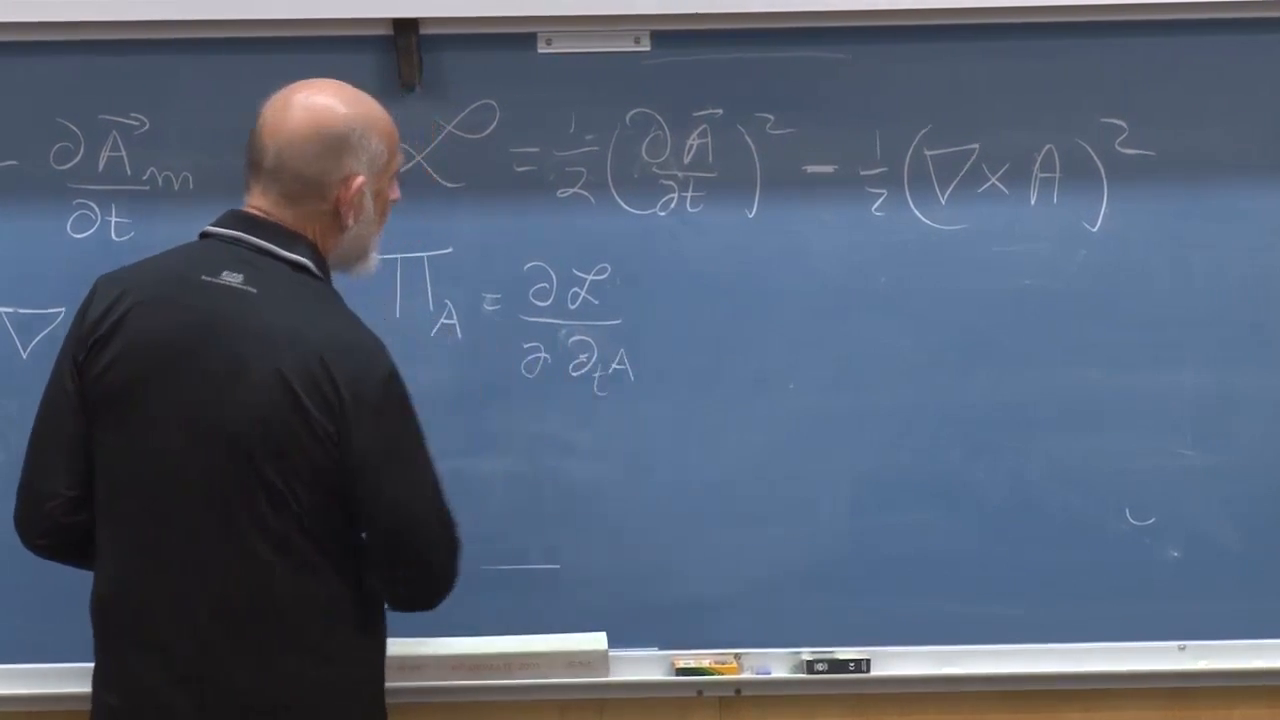
\includegraphics[width=\linewidth]{lecture_10_figure_20.png}
\caption{マクスウェルラグランジアンを、\(\mathbf A\)の空間成分に対する力学的場のラグランジアンとして書き直したもの。}
\par\smallskip
\textit{講義フレーム：01：28：10。}
\end{figure}

各成分\(A_m\)は正準運動量をもち、
\begin{equation}
\Pi_m
 =\frac{\partial\mathcal L_{\mathrm{EM}}}
        {\partial\dot A_m}
 =\dot A_m
 =-E_m.
\label{eq:em-canonical-momentum}
\end{equation}
これはなぜ規約が重要であるかの具体的な例である。先の逆の電場規約では、正準微分自体は変わらないものの、最後に表示される符号が変わるであろう。

\begin{figure}[H]
\centering
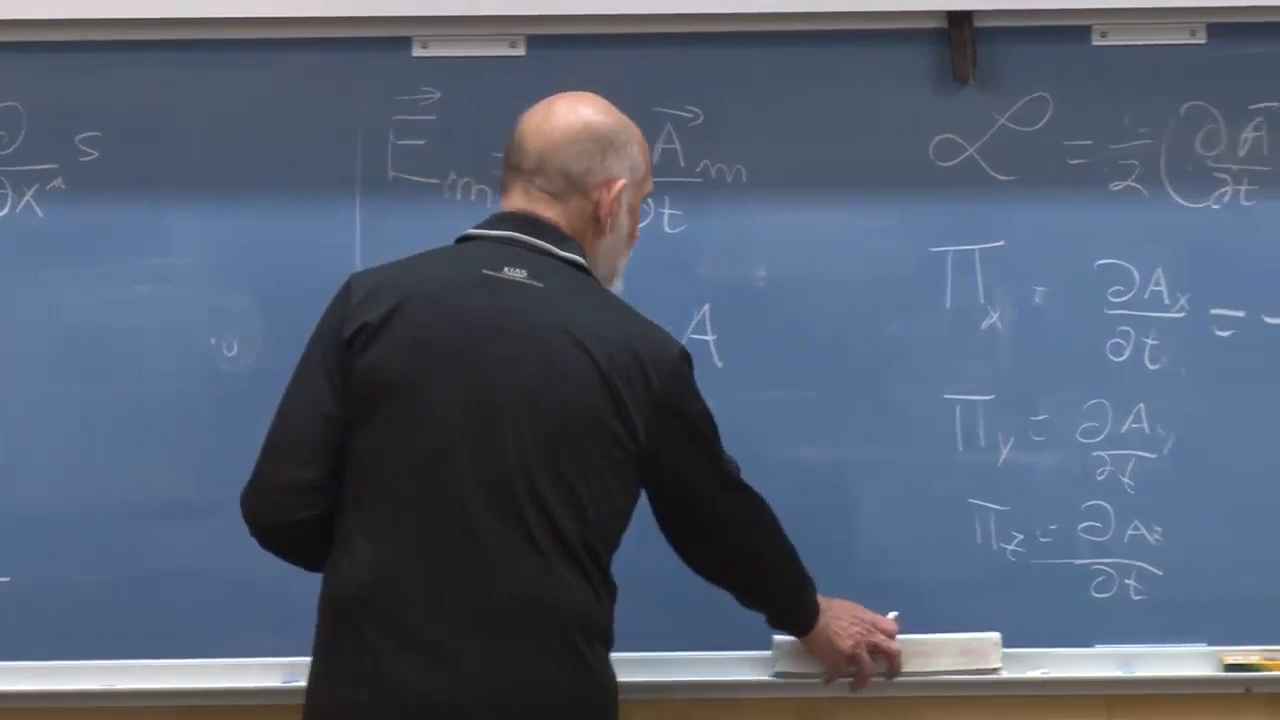
\includegraphics[width=\linewidth]{lecture_10_figure_21.png}
\caption{\(A_x,A_y,A_z\)に対応する3つの正準運動量場は、それぞれ対応する時間微分に等しく、したがって標準的な電場の負に等しい。}
\par\smallskip
\textit{講義フレーム：01：30：20。}
\end{figure}

ハミルトニアンの近道が今や正当化される：時間微分を含まない項の符号を逆にすればよい。電磁気のエネルギー密度は
\begin{equation}
T^{00}_{\mathrm{EM}}
 =\mathcal H_{\mathrm{EM}}
 =\frac12\left(\mathbf E^2+\mathbf B^2\right),
\label{eq:em-energy-density}
\end{equation}
および
\begin{equation}
H_{\mathrm{EM}}
 =\int d^3x\,
\frac12\left(\mathbf E^2+\mathbf B^2\right).
\label{eq:em-total-energy}
\end{equation}
ラグランジアン密度とは異なり、エネルギー密度は非負である。

\begin{figure}[H]
\centering
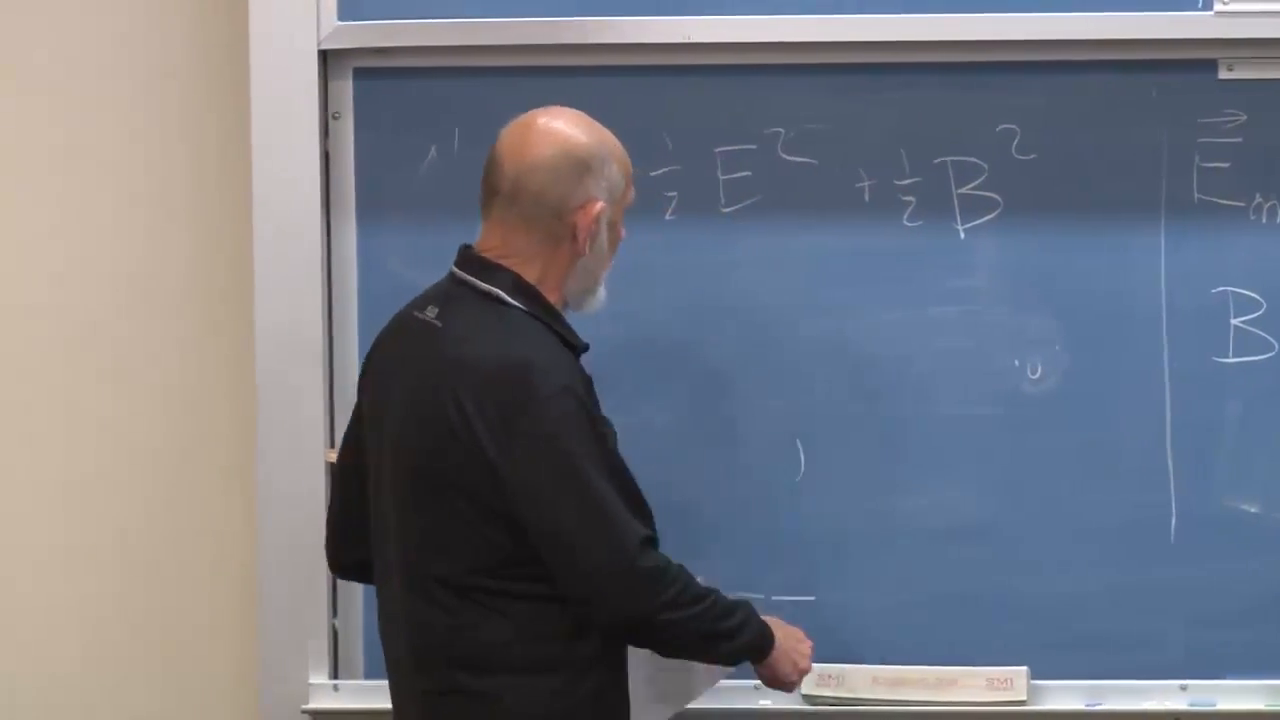
\includegraphics[width=\linewidth]{lecture_10_figure_22.png}
\caption{正の電磁気ハミルトニアン密度\(\frac12(\mathbf E^2+\mathbf B^2)\)。}
\par\smallskip
\textit{講義フレーム：01：32：00。}
\end{figure}

真空中の平面波\(\mathbf E\perp\mathbf B\)では、2つの場は同位相であり、\(c=1\)単位では等しい大きさをもつ。したがって電場と磁場の寄与は波のエネルギーを等しく分け合う：
\begin{equation}
u_E=\frac12\mathbf E^2,
\qquad
u_B=\frac12\mathbf B^2,
\qquad
u_E=u_B.
\label{eq:plane-wave-energy-halves}
\end{equation}

\section{電磁気的運動量の導出}

ネーターの並進公式は今や3つの場\(A_m\)について和をとらなければならない。物理的運動量が波の伝播に沿うように並進の符号を選ぶと、\(n\)成分は
\begin{equation}
P_n
 =\int d^3x\,E_m\,\partial_nA_m,
\label{eq:em-canonical-noether-momentum}
\end{equation}
ここで\(m\)について和をとる。講義はこの符号について意図的に立ち止まる：それは先の電場および能動的／受動的並進の選択に依存する。ゲージ不変な物理的結果がそれを確定するであろう。

\begin{figure}[H]
\centering
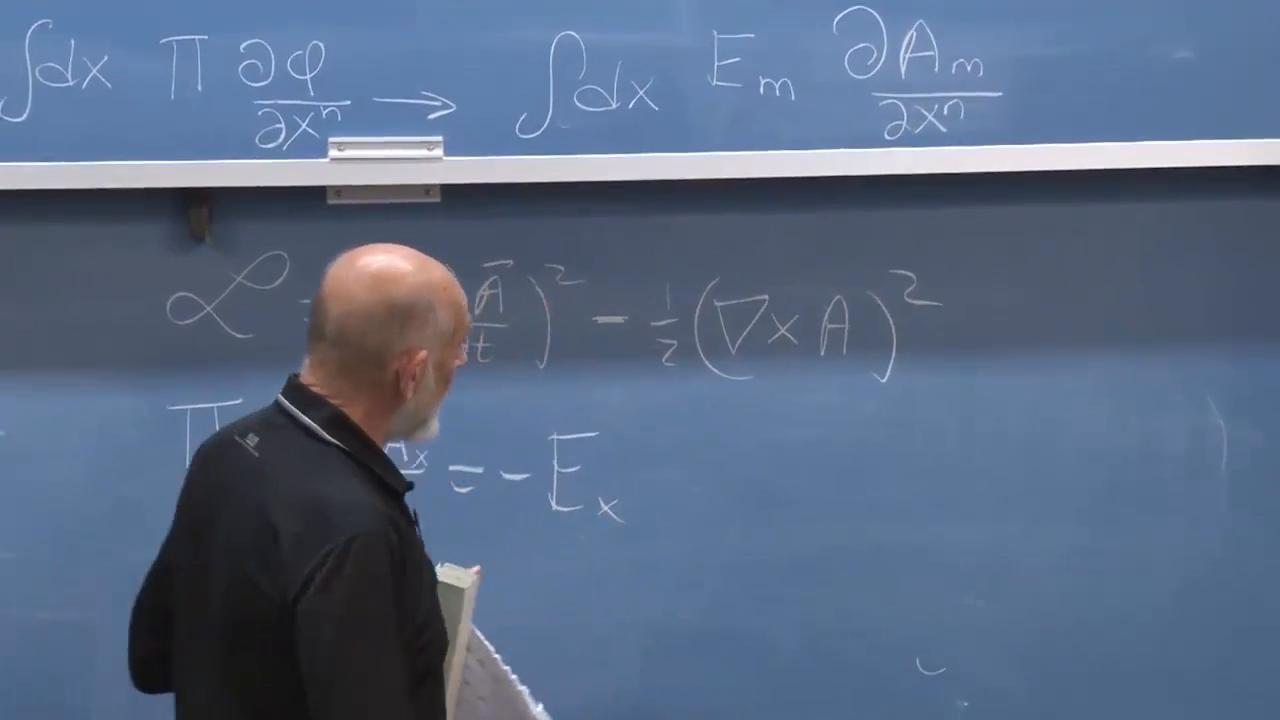
\includegraphics[width=\linewidth]{lecture_10_figure_23.png}
\caption{スカラー場のネーター公式をベクトルポテンシャルの3成分に昇格させたもの。}
\par\smallskip
\textit{講義フレーム：01：36：40。}
\end{figure}

被積分関数は依然として物理的場のみならずゲージポテンシャルを含んでいる。\(E_m\partial_mA_n\)を挿入し、引く：
\begin{align}
E_m\partial_nA_m
 &=
 E_m\left(\partial_nA_m-\partial_mA_n\right)
 +E_m\partial_mA_n.
\label{eq:add-subtract-em-momentum}
\end{align}
第1項はクロス積であり、
\begin{equation}
E_m\left(\partial_nA_m-\partial_mA_n\right)
  =(\mathbf E\times\mathbf B)_n.
\label{eq:cross-product-component}
\end{equation}
第2項は部分積分する：
\begin{align}
\int d^3x\,E_m\partial_mA_n
 &=
\int_{\partial V}d\Sigma_m\,E_mA_n
-\int d^3x\,A_n\partial_mE_m.
\label{eq:em-momentum-integration-parts}
\end{align}
境界項が消えるように場が減衰し、かつ領域が源を含まず
\(\boldsymbol{\nabla}\cdot\mathbf E=0\)であるならば、第2項は何も寄与しない。

\begin{figure}[H]
\centering
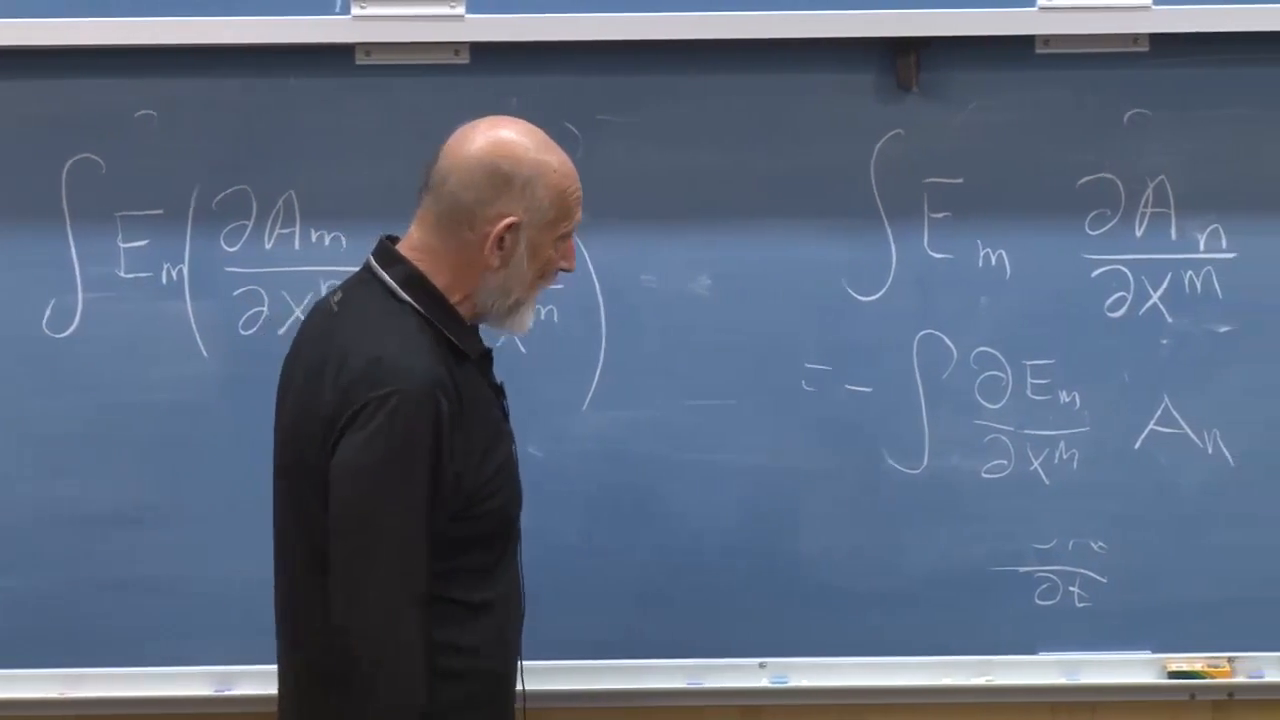
\includegraphics[width=\linewidth]{lecture_10_figure_24.png}
\caption{加えられた項は部分積分により\(\nabla\cdot\mathbf E\)へ移された。}
\par\smallskip
\textit{講義フレーム：01：40：00。}
\end{figure}

したがって全場の運動量は、講義の単位で
\begin{equation}
\mathbf P_{\mathrm{EM}}
 =\int d^3x\,\mathbf E\times\mathbf B,
\qquad
\mathbf g_{\mathrm{EM}}
 =\mathbf E\times\mathbf B,
\label{eq:em-momentum-density}
\end{equation}
である。ベクトル\(\mathbf g_{\mathrm{EM}}\)は電磁気的運動量密度である。

\begin{figure}[H]
\centering
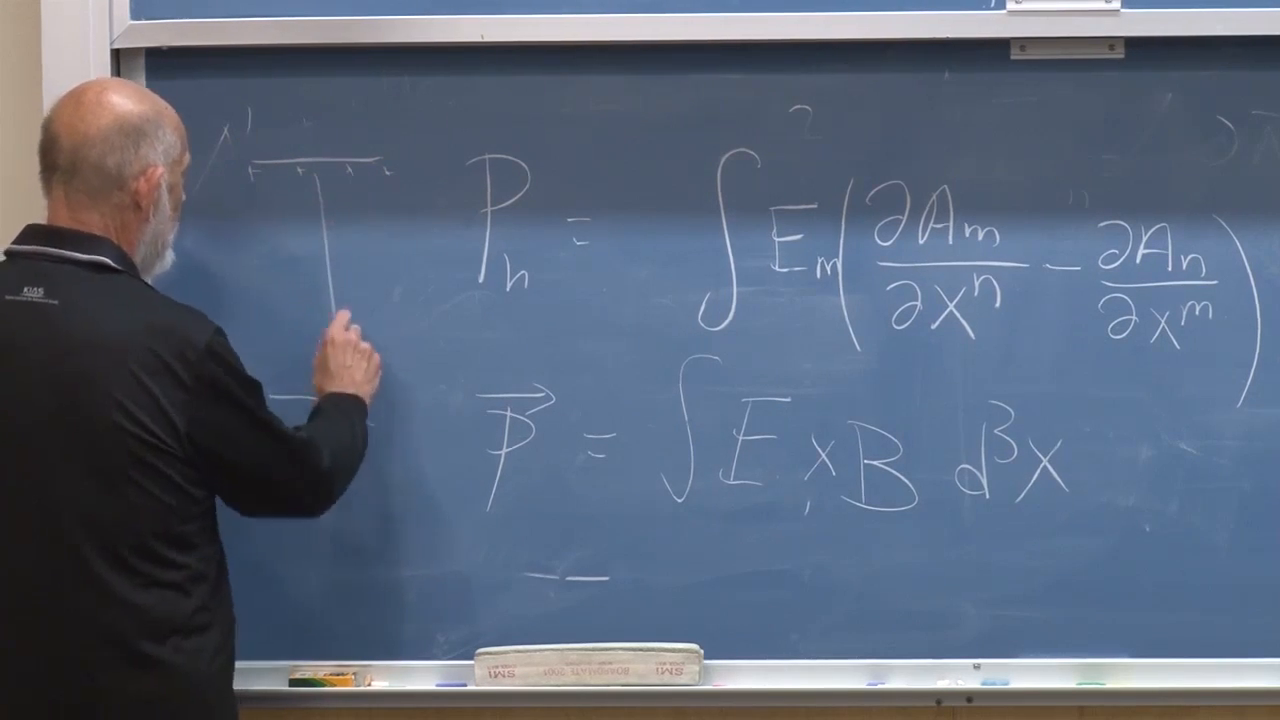
\includegraphics[width=\linewidth]{lecture_10_figure_25.png}
\caption{ゲージポテンシャルの表式はゲージ不変な運動量\(\int d^3x\,\mathbf E\times\mathbf B\)に還元された。}
\par\smallskip
\textit{講義フレーム：01：41：10。}
\end{figure}

\begin{classroomqa}
\audiencequestion{\(\boldsymbol{\nabla}\cdot\mathbf E=0\)はどこで使われたのか、また電荷が存在する場合はどうなるのか。}
\lecturerresponse{それは部分積分の後に体積項を消すので、表示された場のみの導出は自由電磁波に適用される。電荷が存在する場合、その項はゼロではなく、荷電物質の運動量を含めなければならない。並進不変性と運動量保存は完全な物質--場系に関するものである。\lecturetimestamp{01:41:55}}
\end{classroomqa}

\subsection{波の運動量の向き}

平面波では、\(\mathbf E\)、\(\mathbf B\)、および伝播方向が右手系の三つ組をなす。半波長後には\(\mathbf E\)と\(\mathbf B\)の両方が反転する：
\begin{equation}
(-\mathbf E)\times(-\mathbf B)
 =\mathbf E\times\mathbf B.
\label{eq:poynting-sign-reversal}
\end{equation}
したがって運動量密度は振動全体を通じて一つの固定した向き、すなわち波が進む向きを指す。

\begin{figure}[H]
\centering
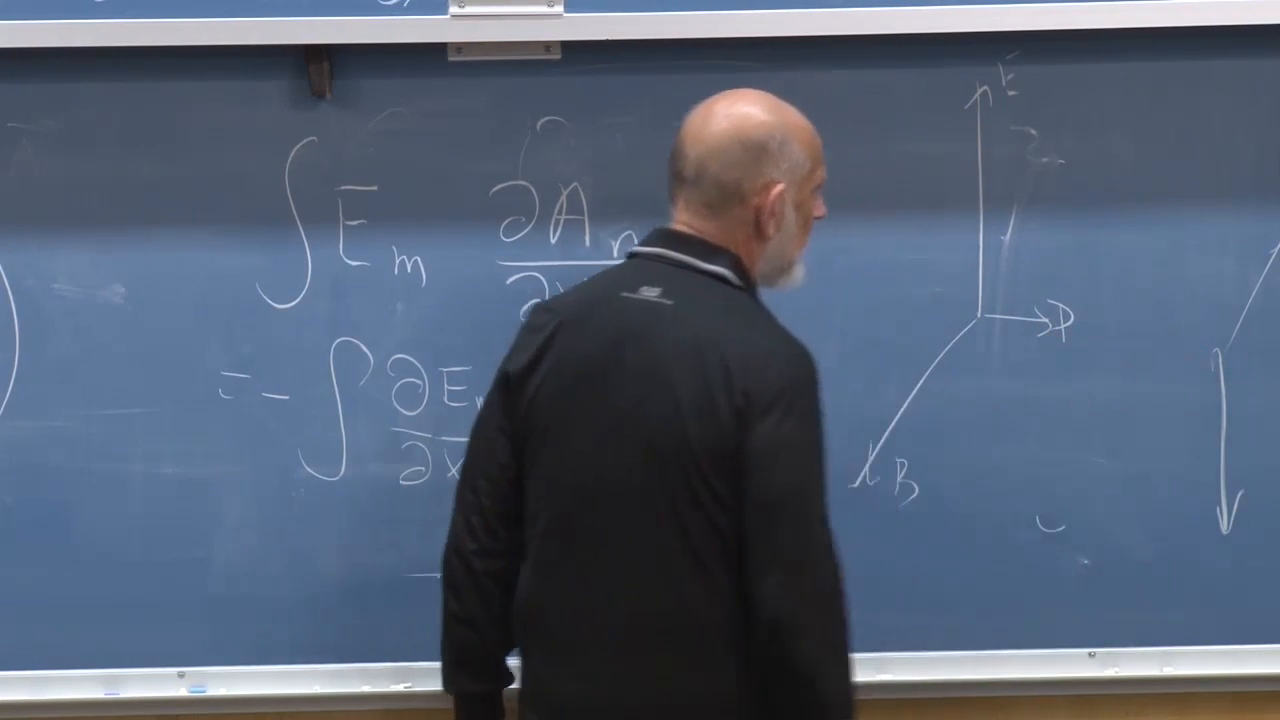
\includegraphics[width=\linewidth]{lecture_10_figure_26.png}
\caption{平面波の幾何：電場と磁場はともに反転するが、それらの外積は伝播軸に沿って進み続ける。}
\par\smallskip
\textit{講義フレーム：01:43:10。}
\end{figure}

これが光圧が実在する理由である。吸収は場の運動量を物質に移す。反射は光の運動量を反転させ、反射体に法線成分の二倍を移すことができる。

\section{ポテンシャルが観測可能な場と出会うところ}

最後に、クラスは\(A_\mu\)と観測可能な場との接点を尋ねる。それらはまさに
\begin{align}
E_n&=-\partial_tA_n+\partial_nA_0,
\nonumber\\
B_n&=\epsilon_{nmk}\partial_mA_k.
\label{eq:potential-field-contact}
\end{align}
時間的ゲージは\(A_0\)項を除去するが、物理的な場を変えない。

\begin{figure}[H]
\centering
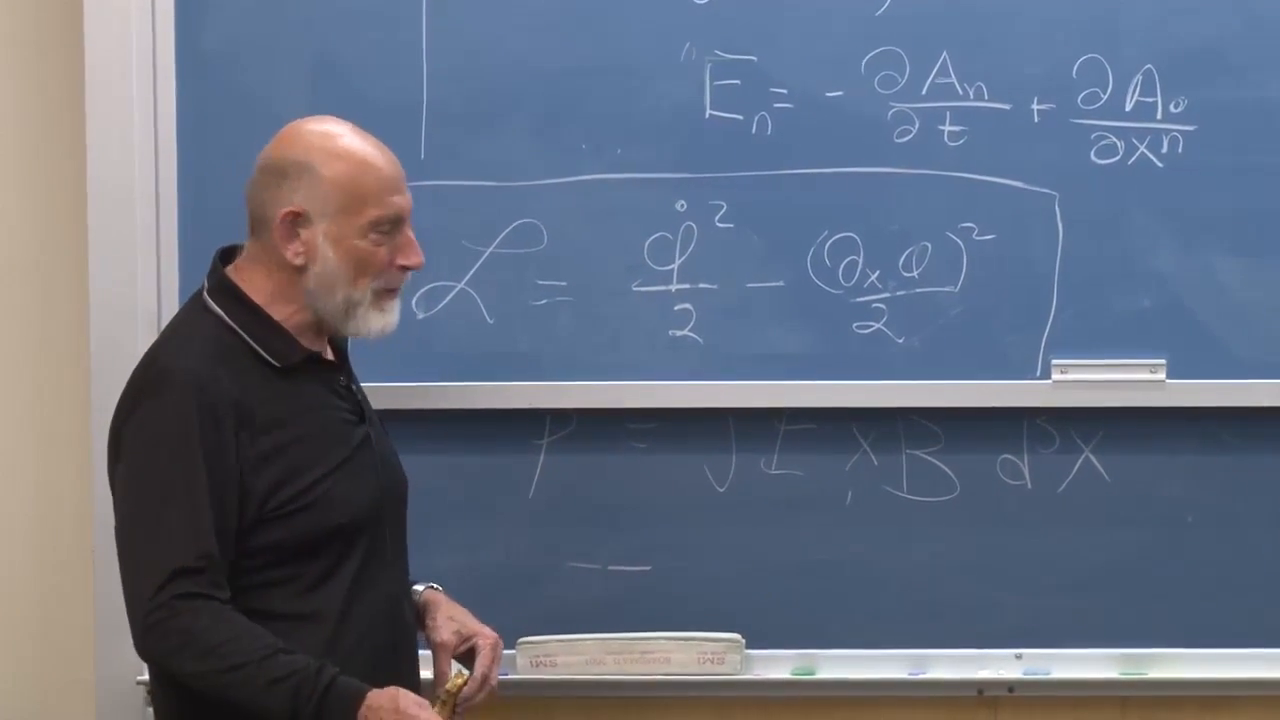
\includegraphics[width=\linewidth]{lecture_10_figure_27.png}
\caption{時間的ゲージの計算の後に復元された一般的な電場の関係、およびその下に想起される共変スカラーラグランジアン。}
\par\smallskip
\textit{講義フレーム：01:45:40。}
\end{figure}

\begin{classroomqa}
\audiencequestion{ベクトルポテンシャルと電場および磁場は正確にどこで結びつくのか。}
\lecturerresponse{電場は空間ポテンシャルの時間微分と\(A_0\)の空間微分を組み合わせる。磁場は空間ポテンシャルの回転である。時間的ゲージではこれは単に
\(\mathbf E=-\dot{\mathbf A}\)および
\(\mathbf B=\nabla\times\mathbf A\)となる。
\lecturetimestamp{01:44:15}}
\end{classroomqa}

\begin{classroomqa}
\audiencequestion{ポテンシャルは\(\mathbf E\)および\(\mathbf B\)よりも基本的なのか。}
\lecturerresponse{作用とゲージ原理は\(A_\mu\)を用いて最も自然に定式化され、それによりポテンシャルは構造的に基本的となる。しかし\(A_\mu\)は一意ではない：ゲージに関連するポテンシャルは同じ物理を表し、局所場はゲージ不変である。二つの主張は両立する。基本的な変数はそれ自体が直接観測可能である必要はない。\lecturetimestamp{01:46:36}}
\end{classroomqa}

\begin{classroomqa}
\audiencequestion{ゲージポテンシャル自体が力を及ぼすことができるのか。}
\lecturerresponse{ゲージに依存する代表はゲージに依存する可測な力を生み出せない。荷電物質は作用の中でポテンシャルを通じて結合されるが、古典的なローレンツ力はゲージ不変な電場と磁場のみで完全に書き表せる。\lecturetimestamp{01:47:49}}
\end{classroomqa}

\begin{classroomqa}
\audiencequestion{交差した電場と磁場が静的であるなら、それらの運動量はゼロでなければならないのか。}
\lecturerresponse{場それ自体については必ずしもそうではない：
\(\mathbf E\times\mathbf B\)は両方の場が時間に依存しない場合でも非ゼロでありうる。閉じた静的装置では、完全な運動量の収支には電荷、電流、支持体、およびあらゆる力学的または隠れた運動量も含まれる。全体が釣り合わなければならないという短い教室での答えは正しい保存の主張である；場の寄与だけをゼロとすることは強すぎるであろう。
\lecturetimestamp{01:48:01}}
\end{classroomqa}

\section{一つのテンソル、ポインティングベクトルの二つの意味}

エネルギー--運動量テンソルはすべての密度と流束を組織する：
\begin{align}
T^{00}&=\text{energy density},\\
T^{0i}&=\text{\(i\)-momentum density},\\
T^{i0}&=\text{energy flux in the \(i\)-direction},\\
T^{ij}&=\text{\(j\)-momentum flux in the \(i\)-direction}.
\label{eq:stress-energy-components}
\end{align}
例えば、\(T^{31}\)は法線が\(z\)方向を指す単位面積を単位時間に横切る\(x\)運動量の量である。空間ブロック\(T^{ij}\)は応力テンソルである。

\begin{figure}[H]
\centering
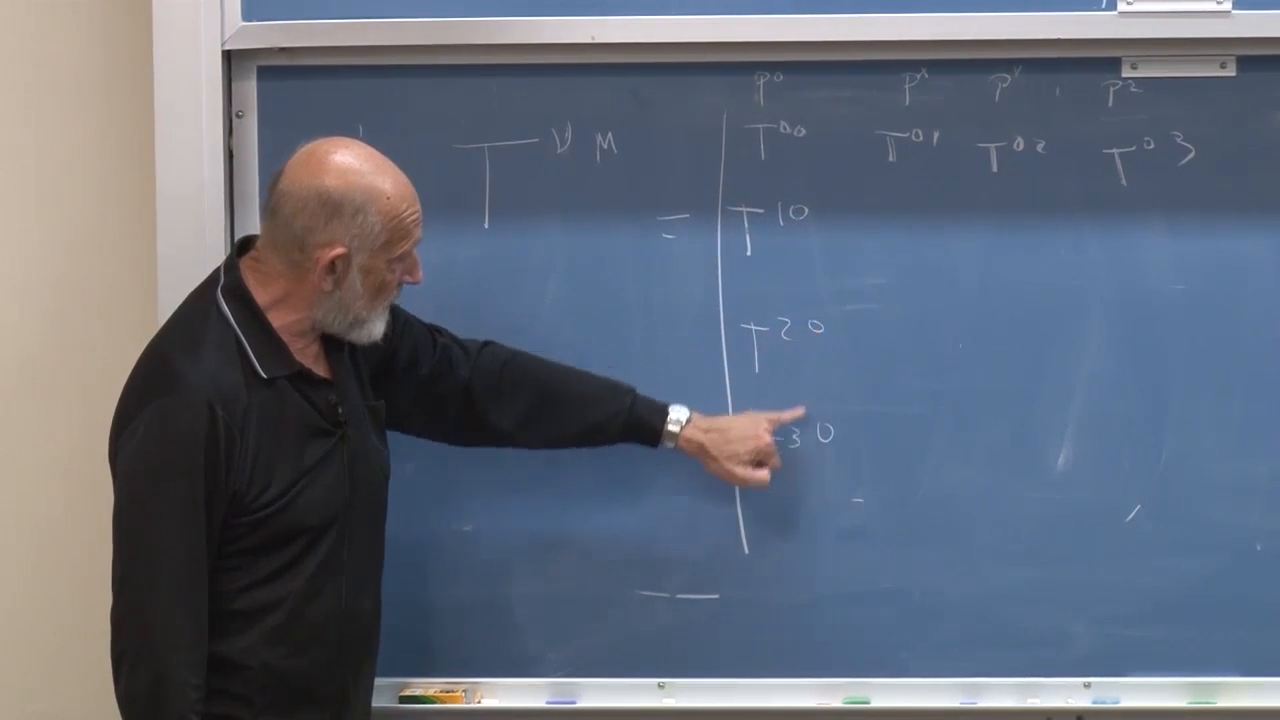
\includegraphics[width=\linewidth]{lecture_10_figure_28.png}
\caption{黒板は密度と流束の成分をエネルギー--運動量テンソルに配列し始める。}
\par\smallskip
\textit{講義フレーム：01:51:10。}
\end{figure}

議論されている相対論的系では、物理的なエネルギー--運動量テンソルは対称に選ぶことができる：
\begin{equation}
T^{\mu\nu}=T^{\nu\mu}.
\label{eq:stress-energy-symmetry}
\end{equation}
したがって、
\begin{equation}
T^{0i}=T^{i0}.
\label{eq:momentum-density-energy-flux}
\end{equation}
\(c=1\)のとき、\(i\)運動量の密度は\(i\)方向のエネルギーの流束に等しい。これが最後の聴衆の記憶への答えである：ポインティングベクトルは確かに電力密度である。

\begin{classroomqa}
\audiencequestion{\(\mathbf E\times\mathbf B\)は、運動量密度ではなく電力密度なのですか。}
\lecturerresponse{その両方である。\(T^{\mu\nu}\)の対称性により、運動量密度\(T^{0i}\)がエネルギー流束\(T^{i0}\)と同一視される。したがって、\(\mathbf S=\mathbf E\times\mathbf B\)は単位時間当たり単位面積当たりのエネルギーであり、\(c=1\)の単位では単位体積当たりの運動量である。通常の単位に戻すと、\(\mathbf g=\mathbf S/c^2\)となる。
\lecturetimestamp{01:48:20}}
\end{classroomqa}

\begin{figure}[H]
\centering
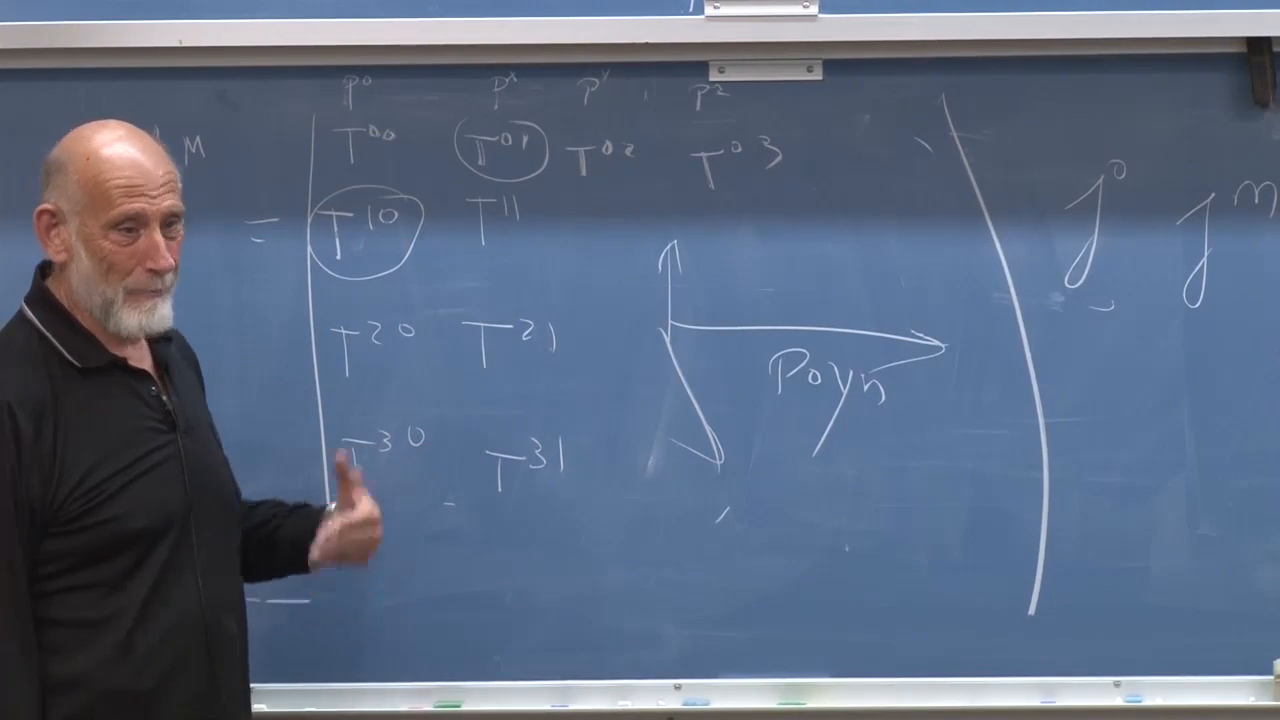
\includegraphics[width=\linewidth]{lecture_10_figure_29.png}
\caption{運動量密度とエネルギー流束を等置する対称テンソルの関係であり、黒板ではポインティング・ベクトルによって表されている。}
\par\smallskip
\textit{講義フレーム：01：53：50。}
\end{figure}

\section{一般相対性理論への橋}

この講義は、古典力学、場の理論、電磁気学を一つの構造にまとめることで締めくくられる：
\begin{enumerate}
\item 時間並進不変性はハミルトニアンとエネルギーを与える。
\item 空間並進不変性はネーター運動量を与える。
\item 離散的な座標を空間的にラベル付けされた場に置き換えることで、和は積分に、保存量は局所密度になる。
\item ゲージ固定は、マクスウェル場の可観測量を変えることなく、その力学的座標を露わにする。
\item マクスウェル・ハミルトニアンは
\(\frac12(\mathbf E^2+\mathbf B^2)\)を与え、一方、空間並進は
\(\mathbf E\times\mathbf B\)を与える。
\item 対称なエネルギー--運動量テンソルは、エネルギー密度、運動量密度、エネルギー流束、応力を統合する。
\end{enumerate}

これが次の段階で必要となる量である。一般相対性理論では、エネルギー--運動量テンソルがアインシュタインの場の方程式における源として現れる。したがって、最終講義は単に電磁気学的な計算を付け加えただけではなく、物質と場が時空にどのように曲がるかを語る言語を準備したのである。
